\section{Computer vision}

\newcommand{\imagenetplot}[1]{
    \begin{tikzpicture}
        \begin{axis}[
            ylabel={Error rate},
            xlabel={Year},
            xtick={2010, 2012, 2014, 2016, 2018, 2020},
            xticklabels={2010, 2012, 2014, 2016, 2018, 2020},
            ytick={0, 10, 20, 30},
            yticklabels={0\%, 10\%, 20\%, 30\%},
            ytick style={draw=none},
            ytick pos=left,
            xtick pos=bottom,
            ymajorgrids=true,
            ymax=29,
            ymin=0,
            xmin=2009,
            xmax=2021,
            width=8cm,
            height=5cm
        ]
            \ifnum#1=0
                \addplot[mark=*, purple,thick] coordinates {
                    (2010, 28.2)
                    (2011, 25.8)
                };
            \fi
            \ifnum#1=1
                \addplot[mark=*, purple,thick] coordinates {
                    (2010, 28.2)
                    (2011, 25.8)
                    (2012, 16.4)
                };
            \fi
            \ifnum#1>1
                \addplot[mark=*, purple,thick] coordinates {
                    (2010, 28.2)
                    (2011, 25.8)
                    (2012, 16.4)
                    (2013, 11.7)
                    (2014, 7.3)
                    (2015, 3.5)
                    (2016, 3.0)
                    (2017, 2.3)
                    (2018, 1.8)
                    (2019, 1.3)
                    (2020, 0.9)
                };
            \fi

            \node[anchor=north, inner sep=5pt] at (axis cs: 2010, 28.2) {
                \small{28.2}
            };
            \node[anchor=north, inner sep=5pt] at (axis cs: 2011, 25.8) {
                \small{25.8}
            };

            \ifnum#1>0
                \node[anchor=north, inner sep=5pt] at (axis cs: 2012, 16.4) {
                    \small{16.4}
                };

                \addplot[densely dotted] coordinates {
                    (2011.5, 30)
                    (2011.5, 0)
                };
            \fi
            \ifnum#1>1
                \node[anchor=north, inner sep=5pt] at (axis cs: 2013, 11.7) {
                    \small{11.7}
                };
                \node[anchor=north, inner sep=5pt] at (axis cs: 2014, 7.3) {
                    \small{7.3}
                };
                \node[anchor=north, inner sep=5pt] at (axis cs: 2015, 3.5) {
                    \small{3.5}
                };
                \node[anchor=south, inner sep=5pt] at (axis cs: 2016, 3.0) {
                    \small{3.0}
                };
                \node[anchor=south, inner sep=5pt] at (axis cs: 2017, 2.3) {
                    \small{2.3}
                };
                \node[anchor=south, inner sep=5pt] at (axis cs: 2018, 1.8) {
                    \small{1.8}
                };
                \node[anchor=south, inner sep=5pt] at (axis cs: 2019, 1.3) {
                    \small{1.3}
                };
                \node[anchor=south, inner sep=5pt] at (axis cs: 2020, 0.9) {
                    \small{\textbf{0.9}}
                };
            \fi
            \ifnum#1>2
                \addplot[dashed, red] coordinates {
                    (2009, 5.1)
                    (2021, 5.1)
                };

                \node[anchor=south east] at (axis cs: 2021, 5.1) {
                    \textcolor{red}{\small{Human level}}
                };
            \fi
        \end{axis}
    \end{tikzpicture}
}

\newsavebox{\imagenetold}
\sbox{\imagenetold}{
    \imagenetplot{0}
}
\newsavebox{\imagenetcnn}
\sbox{\imagenetcnn}{
    \imagenetplot{1}
}
\newsavebox{\imagenetrecent}
\sbox{\imagenetrecent}{
    \imagenetplot{2}
}
\newsavebox{\imagenethuman}
\sbox{\imagenethuman}{
    \imagenetplot{3}
}

\begin{frame}{Image processing: Background}
    \centering
    \begin{tikzpicture}
        \visible<1-2>{
            \node[inner sep=0pt, label=below:\small{Cat}] (img3) at (0, -1) {
                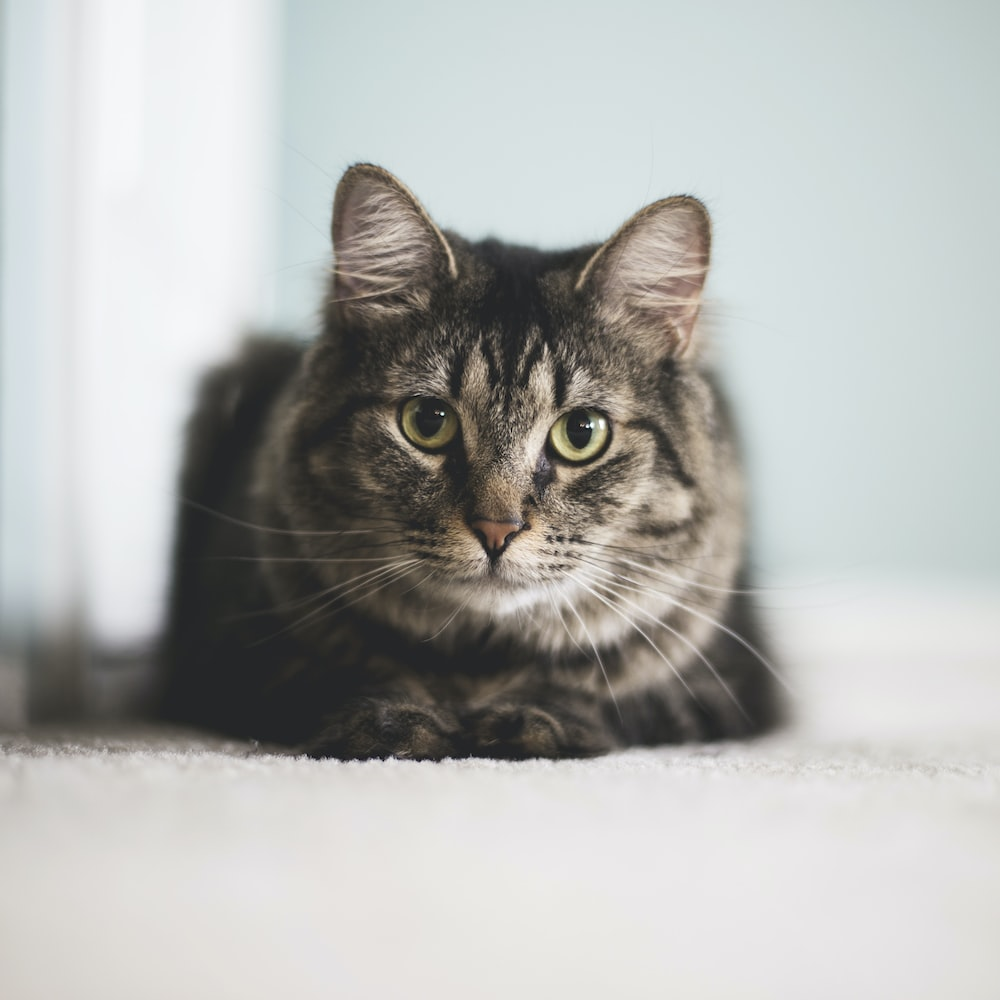
\includegraphics[width=1.5cm]{data/cat.jpeg}
            };
        }
        \visible<2>{
            \node[inner sep=0pt, label=below:\small{Airplane}, anchor=west] (img4) at ($ (img3.east) + (0.1, 0) $) {
                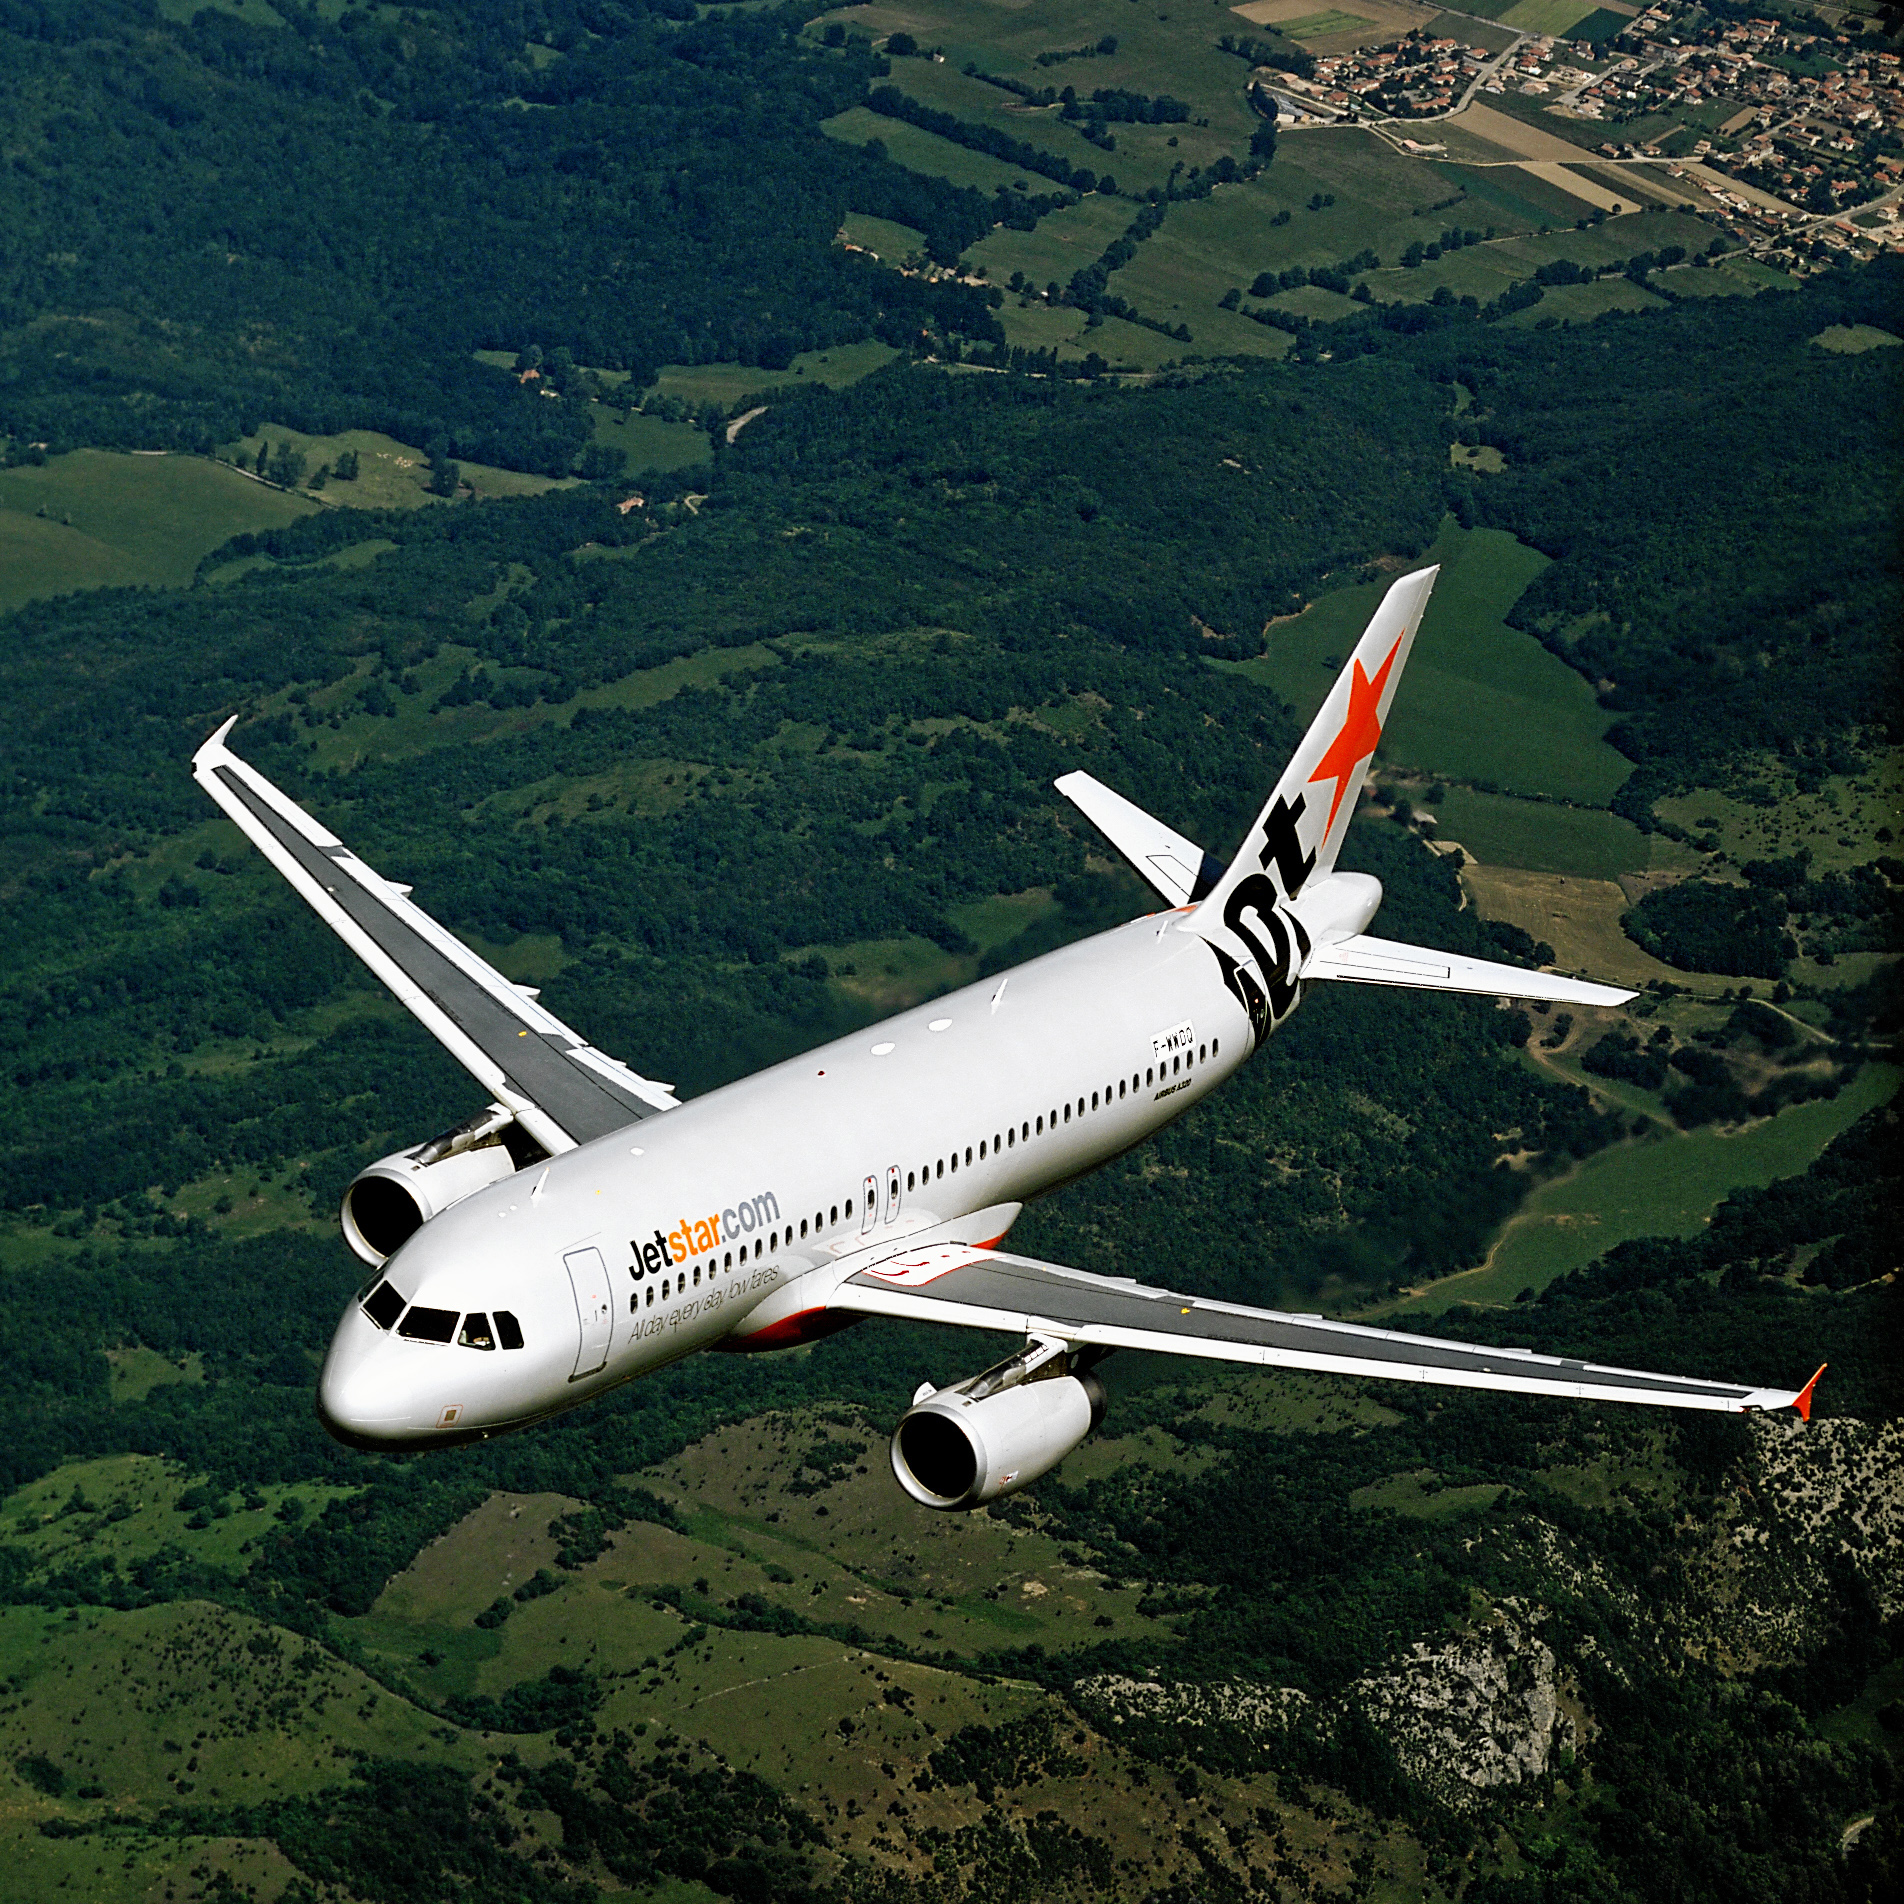
\includegraphics[width=1.5cm]{data/airplane.jpeg}
            };
            \node[inner sep=0pt, label=below:\small{Shark}, anchor=west] (img5) at ($ (img4.east) + (0.1, 0) $) {
                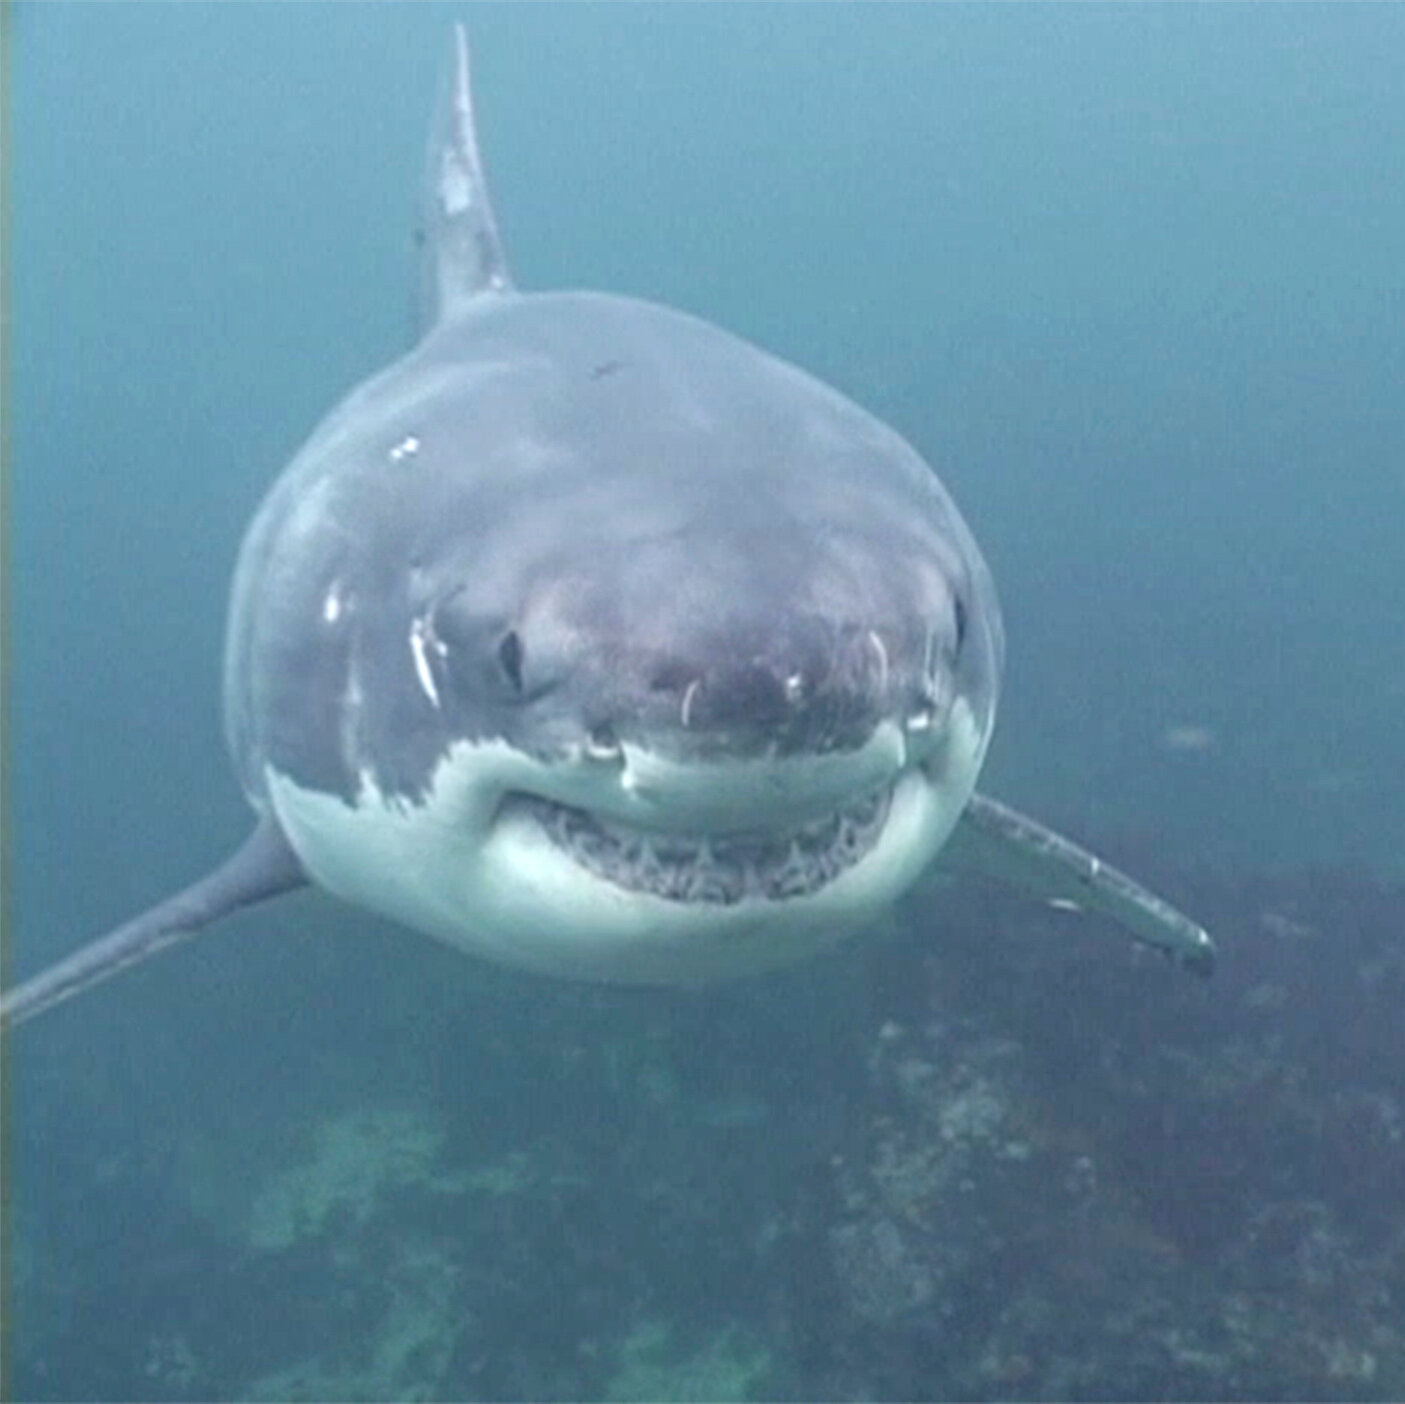
\includegraphics[width=1.5cm]{data/shark.jpeg}
            };
            \node[inner sep=0pt, label=below:\small{Ladybug}, anchor=east] (img2) at ($ (img3.west) - (0.1, 0) $) {
                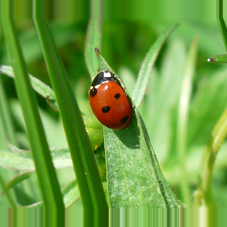
\includegraphics[width=1.5cm]{data/ladybug.png}
            };
            \node[inner sep=0pt, label=below:\small{Sunflower}, anchor=east] (img1) at ($ (img2.west) - (0.1, 0) $) {
                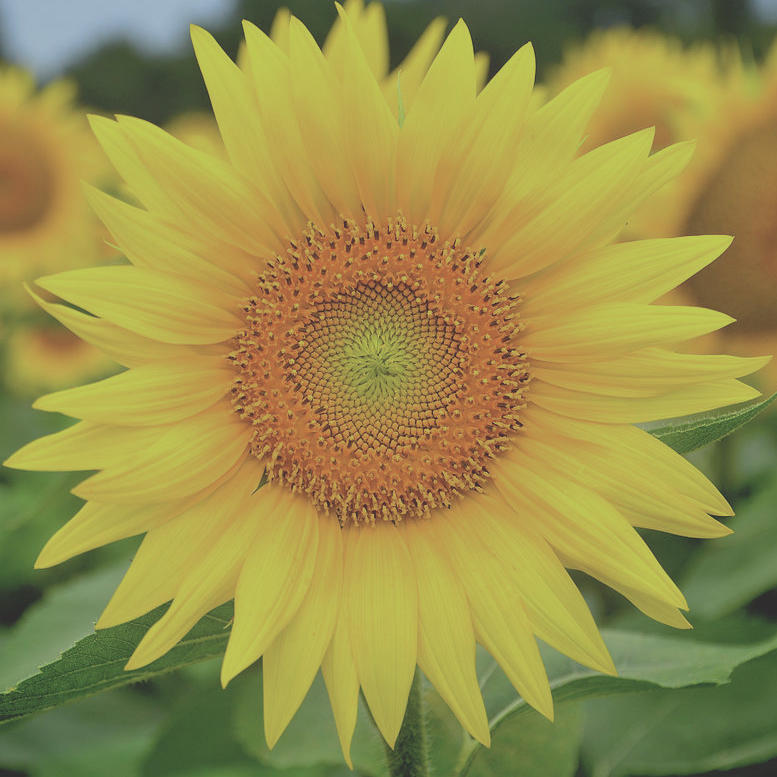
\includegraphics[width=1.5cm]{data/sunflower.jpeg}
            };
            \node[] at (0, -3) {
                ImageNet: $\sim$14m images, $\sim$22k categories
            };
        }
        \visible<3>{
            \node[] at (0, -1) {
                \usebox{\imagenetold}
            };
        }
        \visible<4>{
            \node[] at (0, -1) {
                \usebox{\imagenetcnn}
            };
        }
        \visible<5>{
            \node[] at (0, -1) {
                \usebox{\imagenetrecent}
            };
        }
        \visible<6>{
            \node[] at (0, -1) {
                \usebox{\imagenethuman}
            };
        }
    \end{tikzpicture}
\end{frame}

\begin{frame}{Image processing: Image data}
    \begin{tikzpicture}
        \node[] at (-5.25, 3.5) {};
        \node[] at (5.25, -3.5) {};

        \visible<1-2>{
            \node[draw=black, inner sep=0pt] at (0, 0) {
                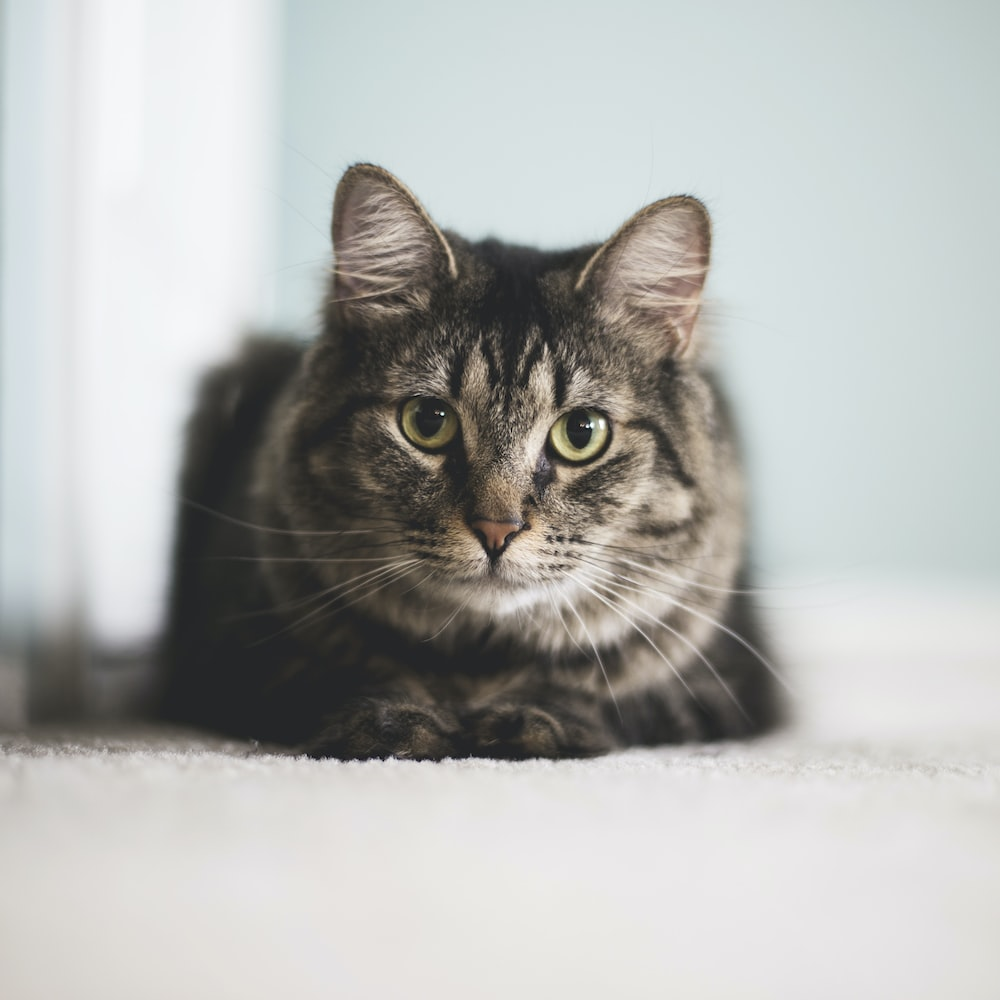
\includegraphics[width=6cm]{data/cat.jpeg}
            };
        }
        \visible<2>{
            \draw[stealth-stealth, red, very thick] (-0.7, 1.5) -- (0.9, 1.3);
        }
        \visible<3-5>{
            \node[draw=black!10, inner sep=0pt] at (0, 0) {
                {\transparent{0.1}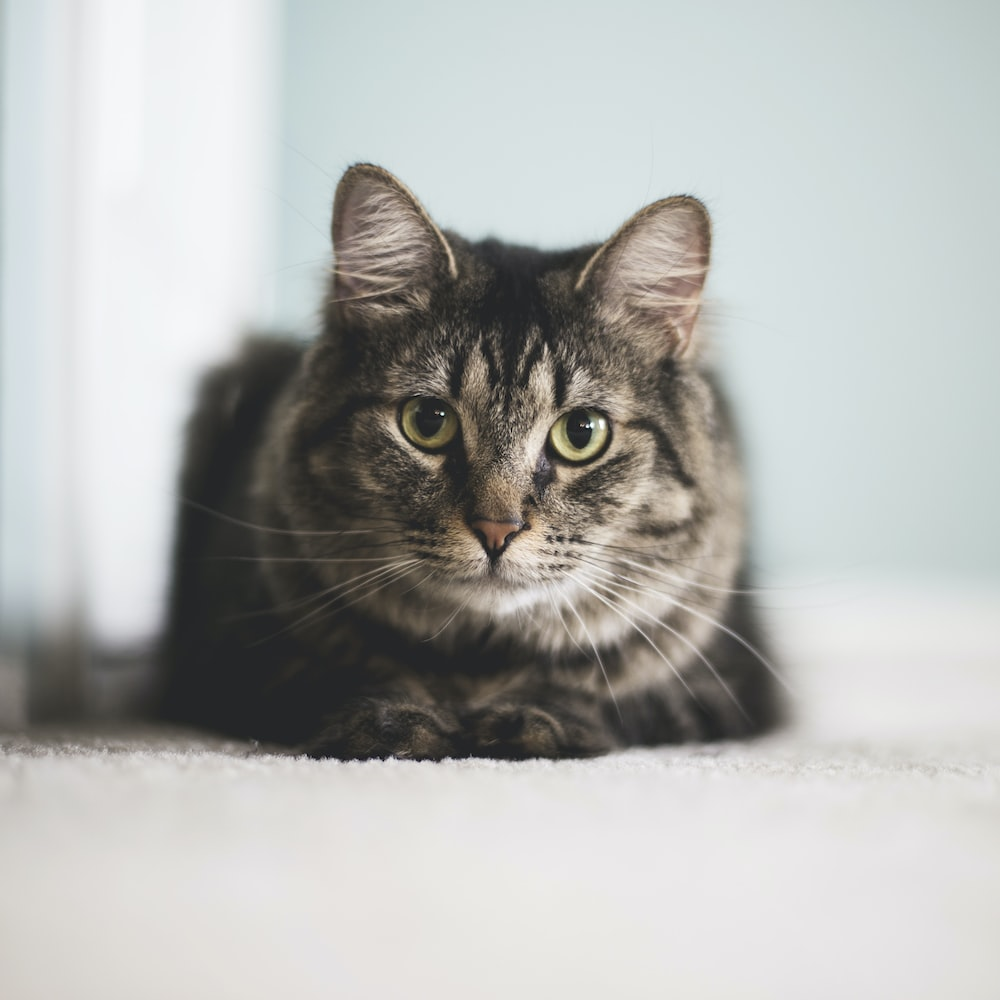
\includegraphics[width=6cm]{data/cat.jpeg}}
            };
        }
        \visible<3>{
            \begin{scope}
                \clip (0.5, 0.4) circle (0.25cm) node {
                    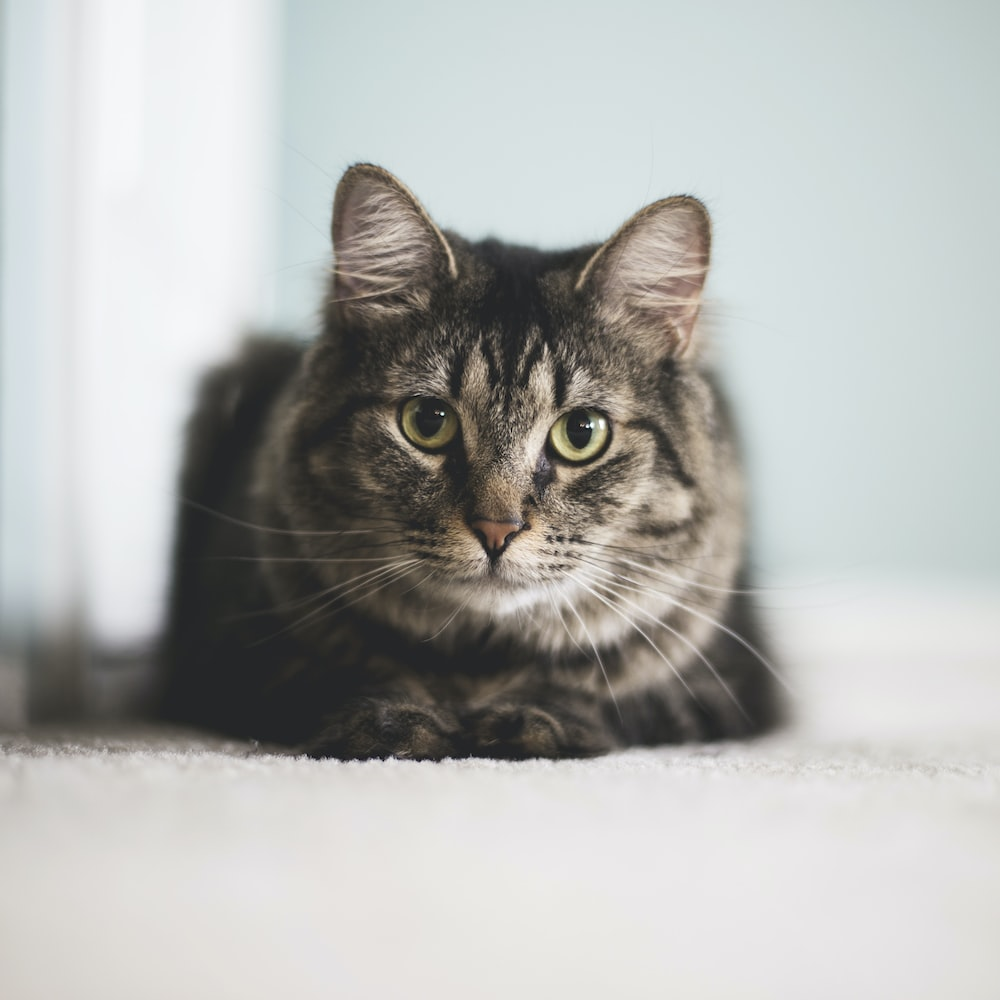
\includegraphics[
                        width=5cm,
                        trim={5.5cm 4.3cm 0 0},
                        clip
                    ]{data/cat.jpeg}
                };
            \end{scope}
        }
        \visible<4>{
            \begin{scope}
                \clip (0, 0) circle (0.9cm) node {
                    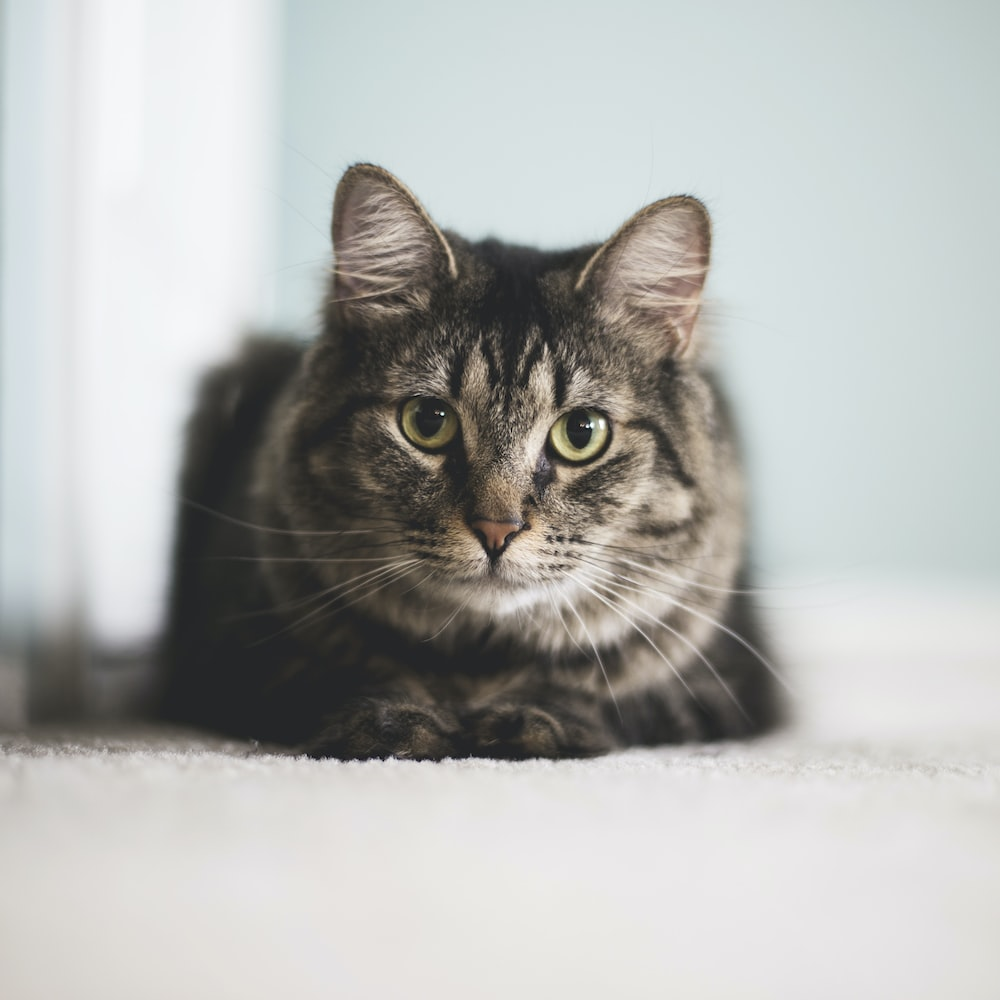
\includegraphics[
                        width=6cm
                    ]{data/cat.jpeg}
                };
            \end{scope}
        }
        \visible<5>{
            \begin{scope}
                \clip (0, 0) circle (2.2cm) node {
                    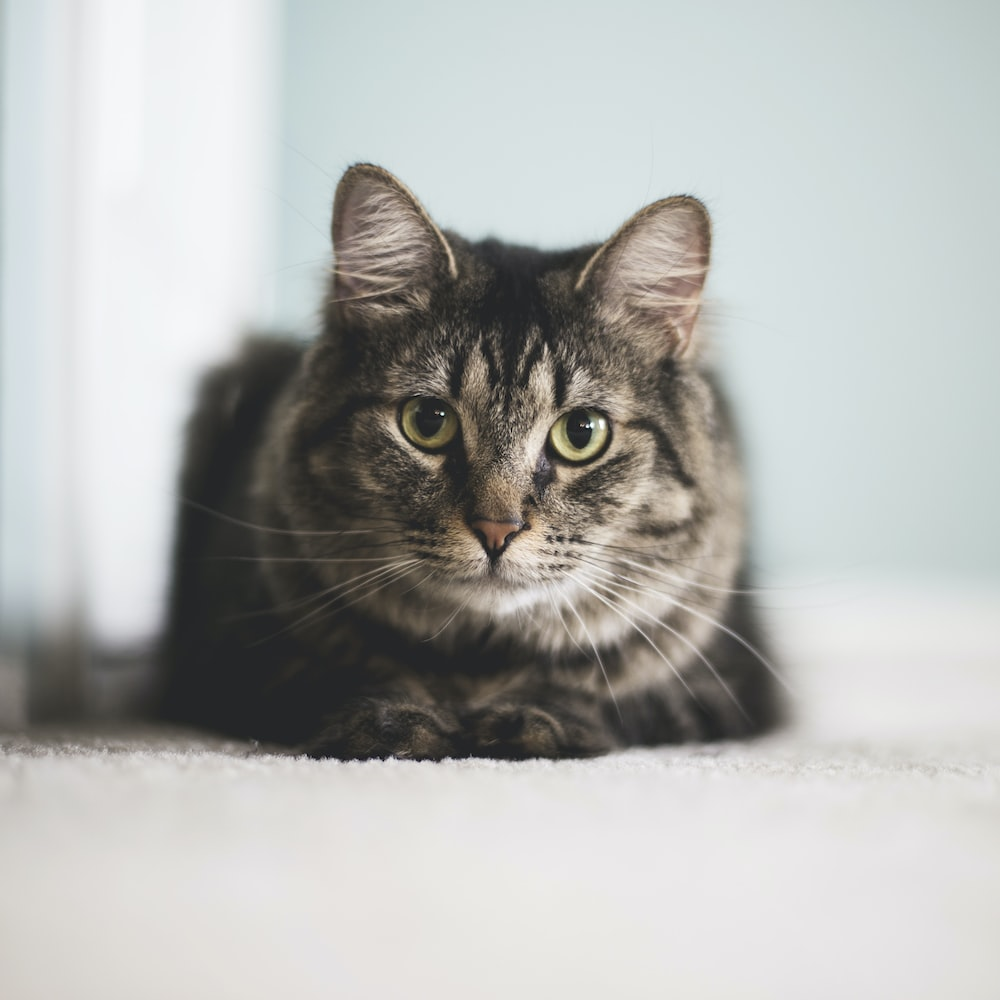
\includegraphics[
                        width=6cm
                    ]{data/cat.jpeg}
                };
            \end{scope}

            \node[circle, minimum size=1.6cm, draw=orange, thick, inner sep=0pt] at (0.03, 0.2) {};
            \node[circle, minimum size=1.1cm, draw=orange, thick, inner sep=0pt] at (-0.7, 1.5) {};
            \node[circle, minimum size=1.1cm, draw=orange, thick, inner sep=0pt] at (0.9, 1.4) {};
        }
        \visible<4-5>{
            \node[circle, minimum size=0.5cm, draw=red, thick, inner sep=0pt] at (0.5, 0.4) {};
            \node[circle, minimum size=0.5cm, draw=red, thick, inner sep=0pt] at (-0.4, 0.45) {};
            \node[circle, minimum size=0.5cm, draw=red, thick, inner sep=0pt] at (-0.03, -0.2) {};
        }
        \visible<6>{
            \node[inner sep=0pt, draw=black] at (-2.5, 0) {
                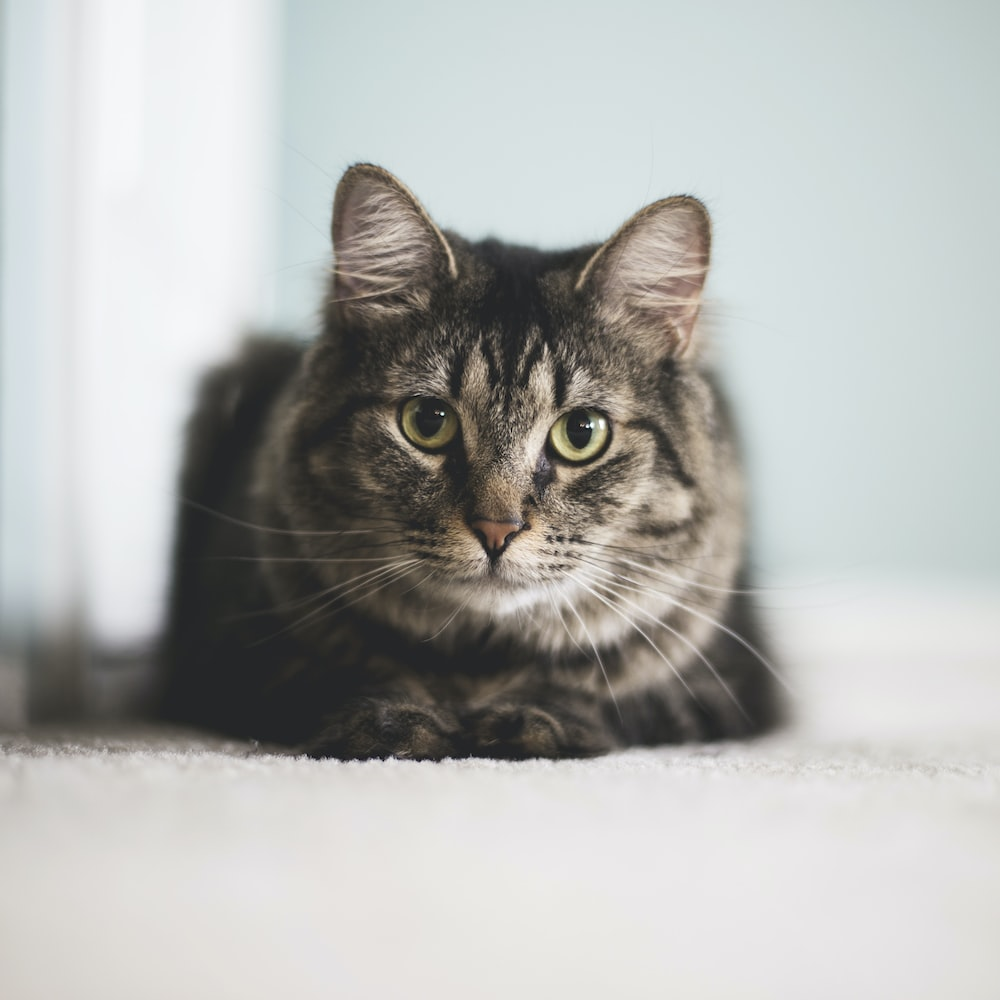
\includegraphics[
                    width=3.5cm,
                    trim={5cm 5cm 0 0},
                    clip
                ]{data/cat.jpeg}
            };
            \node[inner sep=0pt, draw=black] at (2.5, 0) {
                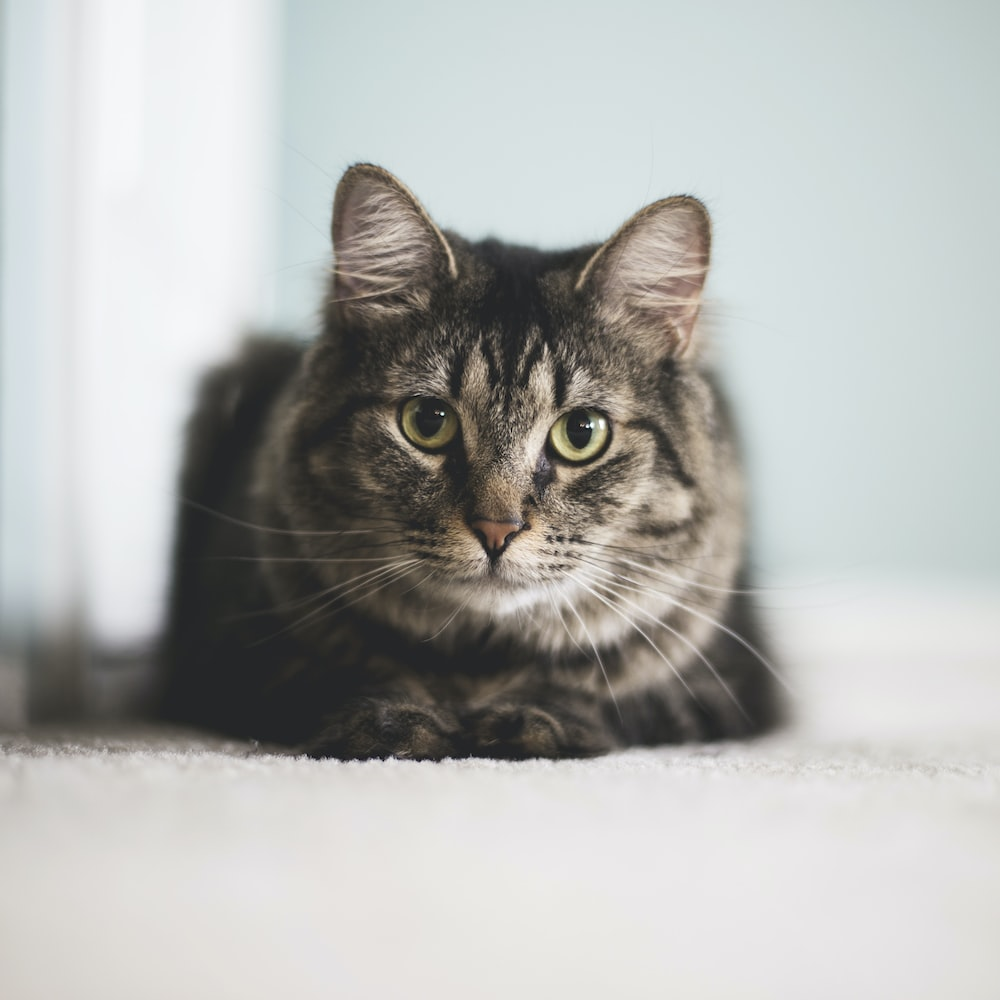
\includegraphics[
                    width=3.5cm,
                    trim={0 0 5cm 5cm},
                    clip
                ]{data/cat.jpeg}
            };
        }
    \end{tikzpicture}
\end{frame}

\begin{frame}{Convolutional neural networks: Inputs}
    \begin{tikzpicture}[ampersand replacement=\&]
        \node[] at (-5.25, 3.25) {};
        \node[] at (5.25, -3.25) {};

        \visible<1-3>{
            \node[
                circle,
                draw=black,
                fill=nodefill,
                minimum size=\nodesize,
                inner sep=0pt,
                text depth=0
            ] (x0) at (-3, 0.5) {\footnotesize{$x_0$}};
            \node[
                circle,
                draw=black,
                fill=nodefill,
                minimum size=\nodesize,
                inner sep=0pt,
                text depth=0
            ] (x1) at (-3, -0.5) {\footnotesize{$x_1$}};
        }
        \visible<1>{
            \artificialneuron{(-1, 1)}{n00}{0}
            \artificialneuron{(-1, 0)}{n01}{0}
            \artificialneuron{(-1, -1)}{n02}{0}

            \artificialneuron{(1, 1)}{n10}{0}
            \artificialneuron{(1, 0)}{n11}{0}
            \artificialneuron{(1, -1)}{n12}{0}

            \node[
                circle,
                draw=black,
                fill=nodefill,
                minimum size=\nodesize,
                inner sep=0pt,
                text depth=0
            ] (y) at (3, 0) {\footnotesize{$\hat{y}$}};

            \draw[->] (x0) -- (n00);
            \draw[->] (x0) -- (n01);
            \draw[->] (x0) -- (n02);
            \draw[->] (x1) -- (n00);
            \draw[->] (x1) -- (n01);
            \draw[->] (x1) -- (n02);

            \draw[->] (n00) -- (n10);
            \draw[->] (n00) -- (n11);
            \draw[->] (n00) -- (n12);
            \draw[->] (n01) -- (n10);
            \draw[->] (n01) -- (n11);
            \draw[->] (n01) -- (n12);
            \draw[->] (n02) -- (n10);
            \draw[->] (n02) -- (n11);
            \draw[->] (n02) -- (n12);

            \draw[->] (n10) -- (y);
            \draw[->] (n11) -- (y);
            \draw[->] (n12) -- (y);

            \draw[->] ($ (n00.north) + (0, 0.3) $) -- (n00.north);
            \draw[->] ($ (n01.north) + (0, 0.3) $) -- (n01.north);
            \draw[->] ($ (n02.north) + (0, 0.3) $) -- (n02.north);
            \draw[->] ($ (n10.north) + (0, 0.3) $) -- (n10.north);
            \draw[->] ($ (n11.north) + (0, 0.3) $) -- (n11.north);
            \draw[->] ($ (n12.north) + (0, 0.3) $) -- (n12.north);
            \draw[->] ($ (y.north) + (0, 0.3) $) -- (y.north);
        }
        \visible<3>{
            \node[] at (-0.6, 0) {
                \Huge{?}
            };
        }
        \visible<3-5>{
            \node[inner sep=0pt, draw=black] (cat) at (3, 0) {
                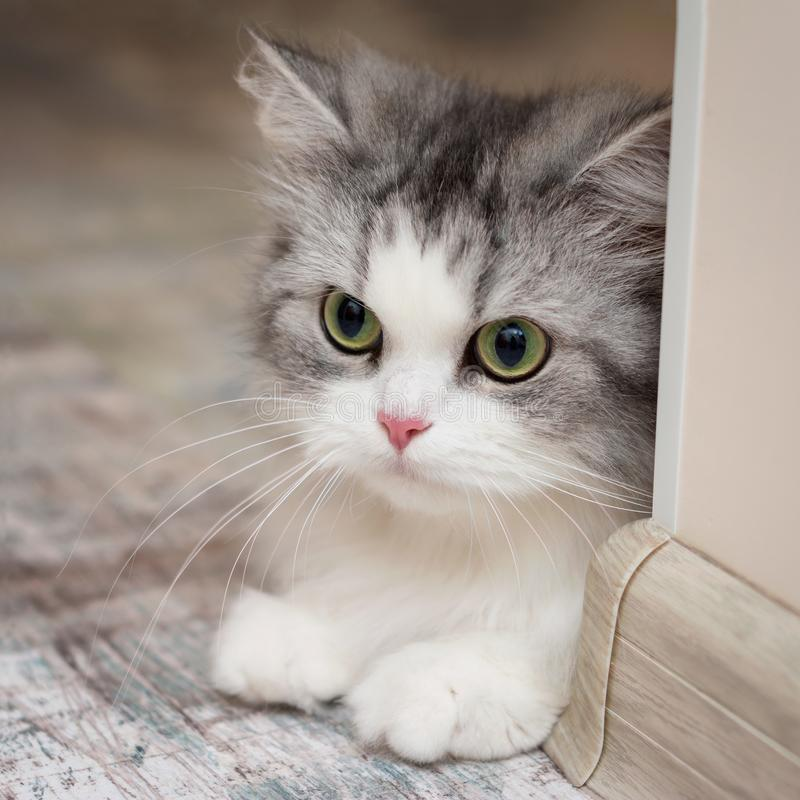
\includegraphics[width=3cm]{data/cat.png}
            };
        }
        \visible<4>{
            \node[] (blue) at (-2.75, -0.25) {
                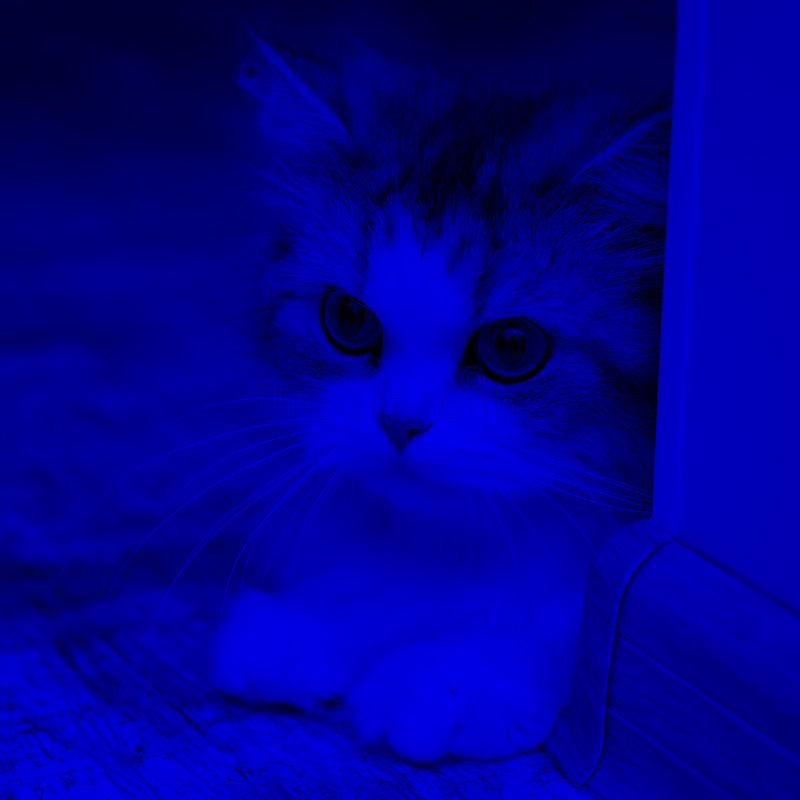
\includegraphics[width=3cm]{data/blue.png}
            };
            \node[] (green) at (-3, 0) {
                
\includegraphics[width=3cm]{data/green.png}
            };
            \node[] (red) at (-3.25, 0.25) {
                
\includegraphics[width=3cm]{data/red.png}
            };

            \draw[<->] ($ (red.north west) - (0.1, 0.1) $) -- ($ (red.south west) - (0.1, -0.1) $) node[midway, above, rotate=90] {\footnotesize{Height}};
            \draw[<->] ($ (blue.south west) - (-0.1, 0.1) $) -- ($ (blue.south east) - (0.1, 0.1) $) node[midway, below] {\footnotesize{Width}};
            \draw[<->] ($ (red.north east) + (-0.1, 0.2) $) -- ($ (blue.north east) + (0.2, -0.1) $) node[midway, above, rotate=315] {\footnotesize{Channels}};
        }
        \visible<4-5>{
            \draw[
                {Stealth[length=5mm]}-{Stealth[length=5mm]},
                line width=5pt,
                gray
            ] ($ (cat.west) + (-0.4, 0) $) -- ($ (green.east) + (0.65, 0) $);
        }
        \visible<5>{
            \matrix[
                matrix of nodes,
                nodes={
                    draw=black,
                    fill=white,
                    minimum width=0.6cm,
                    minimum height=0.6cm,
                    anchor=center,
                    font=\fontsize{4.5}{4.5}\selectfont
                },
                row sep=0cm,
                column sep=0cm
            ]  at (-2.75, -0.25) {
                $x_{002}$ \& $x_{012}$ \& $x_{022}$ \& $x_{032}$ \& $x_{042}$ \\
                $x_{102}$ \& $x_{112}$ \& $x_{122}$ \& $x_{132}$ \& $x_{142}$ \\
                $x_{202}$ \& $x_{212}$ \& $x_{222}$ \& $x_{232}$ \& $x_{242}$ \\
                $x_{302}$ \& $x_{312}$ \& $x_{322}$ \& $x_{332}$ \& $x_{342}$ \\
                $x_{402}$ \& $x_{412}$ \& $x_{422}$ \& $x_{432}$ \& $x_{442}$ \\
            };
            \matrix[
                matrix of nodes,
                nodes={
                    draw=black,
                    fill=white,
                    minimum width=0.6cm,
                    minimum height=0.6cm,
                    anchor=center,
                    font=\fontsize{4.5}{4.5}\selectfont
                },
                row sep=0cm,
                column sep=0cm
            ]  at (-3, 0) {
                $x_{001}$ \& $x_{011}$ \& $x_{021}$ \& $x_{031}$ \& $x_{041}$ \\
                $x_{101}$ \& $x_{111}$ \& $x_{121}$ \& $x_{131}$ \& $x_{141}$ \\
                $x_{201}$ \& $x_{211}$ \& $x_{221}$ \& $x_{231}$ \& $x_{241}$ \\
                $x_{301}$ \& $x_{311}$ \& $x_{321}$ \& $x_{331}$ \& $x_{341}$ \\
                $x_{401}$ \& $x_{411}$ \& $x_{421}$ \& $x_{431}$ \& $x_{441}$ \\
            };
            \matrix[
                matrix of nodes,
                nodes={
                    draw=black,
                    fill=white,
                    minimum width=0.6cm,
                    minimum height=0.6cm,
                    anchor=center,
                    font=\fontsize{4.5}{4.5}\selectfont
                },
                row sep=0cm,
                column sep=0cm
            ]  at (-3.25, 0.25) {
                $x_{000}$ \& $x_{010}$ \& $x_{020}$ \& $x_{030}$ \& $x_{040}$ \\
                $x_{100}$ \& $x_{110}$ \& $x_{120}$ \& $x_{130}$ \& $x_{140}$ \\
                $x_{200}$ \& $x_{210}$ \& $x_{220}$ \& $x_{230}$ \& $x_{240}$ \\
                $x_{300}$ \& $x_{310}$ \& $x_{320}$ \& $x_{330}$ \& $x_{340}$ \\
                $x_{400}$ \& $x_{410}$ \& $x_{420}$ \& $x_{430}$ \& $x_{440}$ \\
            };
        }
    \end{tikzpicture}
\end{frame}

\def\nodesize{14pt}
\colorlet{nodefill}{teal!40}

\newcommand{\cnnchannel}[4]{
    \def\cellsize{0.15}
    \foreach \i in {1,...,#3} {
        \foreach \j in {1,...,#3} {
            \pgfmathsetmacro{\ioffset}{(\i - floor(#3 / 2))}
            \pgfmathsetmacro{\joffset}{(\j - floor(#3 / 2))}
            \node[
                draw=black,
                fill=teal!40,
                minimum width=\cellsize cm,
                minimum height=\cellsize cm,
                anchor=south east,
                inner sep=0pt
            ] (#4\i\j) at ({#1 - (\ioffset * \cellsize)}, {#2 - (\joffset * \cellsize)}) {};

        }
    }
}

\newcommand{\cnnlayer}[5]{
    \pgfmathsetmacro{\rounded}{floor(#4 / 2)}
    \message{\rounded}
    \foreach \c in {1,...,#4} {
        \pgfmathsetmacro{\offset}{\c - 1 - \rounded}
        \cnnchannel{#1 + \offset * 0.1}{#2 - \offset * 0.1}{#3}{#5\c}
    }
}

\begin{frame}{Convolutional neural networks: Architecture}
    \centering
    \resizebox{\textwidth}{!}{
        \begin{tikzpicture}
            \node[inner sep=0pt, draw=black] (cat) at (0, 0) {
                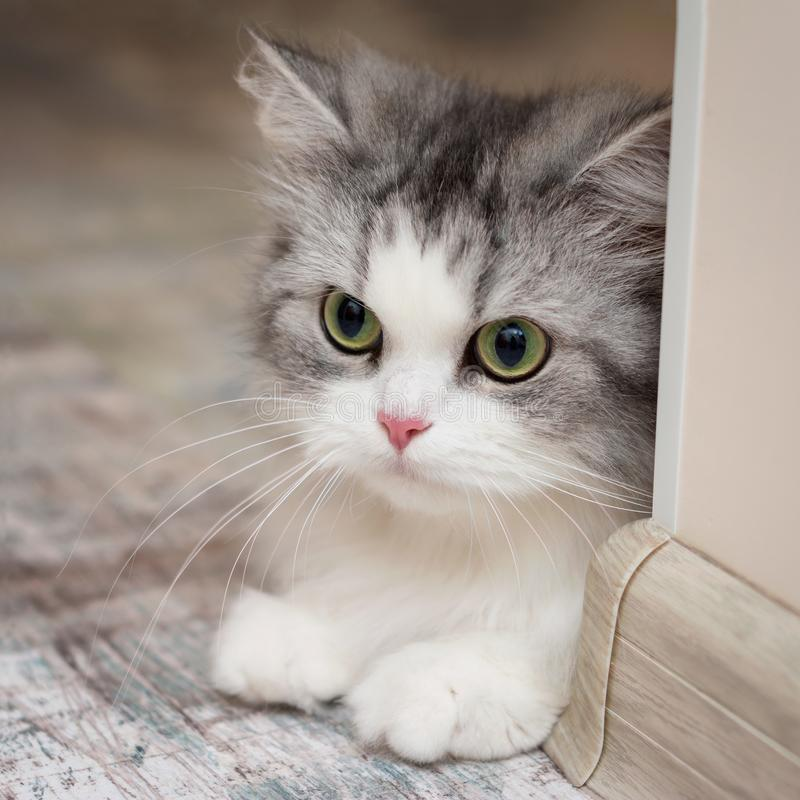
\includegraphics[width=1cm]{data/cat.png}
            };

            \cnnlayer{1.36+0.3}{0}{8}{3}{n1}
            \draw[-stealth] (cat) -- ($ (n1284.south west) - (0.1, 0) $);
            \cnnlayer{2.92+0.3}{0}{6}{3}{n2}
            \draw[-stealth] ($ (n1214.south east) + (0.1, 0) $) -- ($ (n2263.south west) - (0.1, 0) $);
            \cnnlayer{4.43+0.3}{0}{6}{5}{n3}
            \draw[-stealth] ($ (n2213.south east) + (0.1, 0) $) -- ($ (n3363.south west) - (0.2, 0) $);
            \cnnlayer{5.89+0.3}{0}{4}{5}{n4}
            \draw[-stealth] ($ (n3313.south east) + (0.2, 0) $) -- ($ (n4342.south west) - (0.2, 0) $);
            \cnnlayer{7.3+0.3}{0}{4}{7}{n5}
            \draw[-stealth] ($ (n4312.south east) + (0.2, 0) $) -- ($ (n5442.south west) - (0.3, 0) $);
            \cnnlayer{8.66}{0.15}{1}{7}{n6}
            \draw[-stealth] ($ (n5412.south east) + (0.3, 0) $) -- ($ (n6411.south west) - (0, 0) $);

            \node[circle, draw=black, fill=nodefill, text depth=0, inner sep=2pt] (y1) at (9.32, 0.275) {\tiny{$y_0$}};
            \node[circle, draw=black, fill=nodefill, text depth=0, inner sep=2pt] (y2) at (9.57, 0.025) {\tiny{$y_1$}};

            \foreach \n in {1,...,7}{
                \draw[-stealth] (n6\n11) -- (y1);
                \draw[-stealth] (n6\n11) -- (y2);
            }

            \visible<2>{
                \def\operationfont{\scriptsize}
                \node[text depth=0, font=\operationfont\selectfont, anchor=north] at ($(cat)!0.5!(n1244) + (0, -0.8) $) {Convolution};
                \node[text depth=0, font=\operationfont\selectfont, align=center, anchor=north] at ($(n1244)!0.5!(n2233) + (0, -0.8) $) {Pooling};
                \node[text depth=0, font=\operationfont\selectfont, anchor=north] at ($(n2233)!0.5!(n3333) + (0, -0.8) $) {Convolution};
                \node[text depth=0, font=\operationfont\selectfont, align=center, anchor=north] at ($(n3333)!0.5!(n4322) + (0, -0.8) $) {Pooling};
                \node[text depth=0, font=\operationfont\selectfont, anchor=north] at ($(n4322)!0.5!(n5422) + (0, -0.8) $) {Convolution};
                \node[text depth=0, font=\operationfont\selectfont, align=center, anchor=north] at ($(n5422)!0.5!(n6411) + (0, -0.8) $) {Pooling};
            }
        \end{tikzpicture}
    }
    \vfill
\end{frame}

\begin{frame}{Convolutional neural networks: Convolution}
    \centering
    \vfill
    \begin{tikzpicture}[
        ampersand replacement=\&
    ]
        \matrix[
            every node/.style={
                minimum height=0.6cm,
                minimum width=0.6cm,
                draw=black
            },
            label=\footnotesize{Image}
        ] (image) at (0, 0) {
            \only<3>{\node[draw=red,fill=white]{};}
            \only<1-2,4->{\node[fill=white]{};} \&
            \only<3-4>{\node[draw=red,fill=black] {};}
            \only<1-2,5->{\node[fill=black] {};} \&
            \only<3-5>{\node[draw=red,fill=black] {};}
            \only<1-2,6->{\node[fill=black] {};} \&
            \only<4-5>{\node[draw=red,fill=black] {};}
            \only<1-3,6->{\node[fill=black] {};} \&
            \only<5>{\node[draw=red,fill=white] {};}
            \only<1-4,6->{\node[fill=white] {};}\\

            \only<3,6>{\node[draw=red,fill=black] {};}
            \only<1-2,4-5,7->{\node[fill=black] {};}  \&
            \only<3-4,6>{\node[draw=red,fill=white] {};}
            \only<1-2,5,7->{\node[fill=white] {};} \&
            \only<3-6>{\node[draw=red,fill=black] {};}
            \only<1-2,7->{\node[fill=black] {};} \&
            \only<4-5>{\node[draw=red,fill=white] {};}
            \only<1-3,6->{\node[fill=white] {};} \&
            \only<5>{\node[draw=red,fill=black] {};}
            \only<1-4,6->{\node[fill=black] {};} \\

            \only<3,6>{\node[draw=red,fill=black] {};}
            \only<1-2,4-5,7->{\node[fill=black] {};} \&
            \only<3-4,6>{\node[draw=red,fill=black] {};}
            \only<1-2,5,7->{\node[fill=black] {};} \&
            \only<3-6>{\node[draw=red,fill=white] {};}
            \only<1-2,7->{\node[fill=white] {};} \&
            \only<4-5>{\node[draw=red,fill=black] {};}
            \only<1-3,6->{\node[fill=black] {};} \&
            \only<5>{\node[draw=red,fill=black] {};}
            \only<1-4,6->{\node[fill=black] {};} \\

            \only<6>{\node[draw=red,fill=black] {};}
            \only<1-5,7->{\node[fill=black] {};} \&
            \only<6>{\node[draw=red,fill=white] {};}
            \only<1-5,7->{\node[fill=white] {};} \&
            \only<6>{\node[draw=red,fill=black] {};}
            \only<1-5,7->{\node[fill=black] {};} \&
            \node[fill=white] {}; \&
            \node[fill=black] {}; \\

            \node[fill=white] {}; \&
            \node[fill=black] {}; \&
            \node[fill=black] {}; \&
            \node[fill=black] {}; \&
            \node[fill=white] {}; \\
        };

        \visible<2->{
            \matrix[
                every node/.style={
                    minimum height=0.6cm,
                    minimum width=0.6cm,
                    draw=black
                },
                label=below:\footnotesize{Pattern 1}] (kernel1) at (-2.25, -3) {
                \only<3-6>{\node[draw=red,fill=white] {};}
                \only<2,7->{\node[fill=white] {};} \&
                \only<3-6>{\node[draw=red,fill=black] {};}
                \only<2,7->{\node[fill=black] {};} \&
                \only<3-6>{\node[draw=red,fill=black] {};}
                \only<2,7->{\node[fill=black] {};} \\

                \only<3-6>{\node[draw=red,fill=black] {};}
                \only<2,7->{\node[fill=black] {};} \&
                \only<3-6>{\node[draw=red,fill=white] {};}
                \only<2,7->{\node[fill=white] {};} \&
                \only<3-6>{\node[draw=red,fill=black] {};}
                \only<2,7->{\node[fill=black] {};} \\

                \only<3-6>{\node[draw=red,fill=black] {};}
                \only<2,7->{\node[fill=black] {};} \&
                \only<3-6>{\node[draw=red,fill=black] {};}
                \only<2,7->{\node[fill=black] {};} \&
                \only<3-6>{\node[draw=red,fill=white] {};}
                \only<2,7->{\node[fill=white] {};} \\
            };
        }
        \visible<3->{
            \matrix[
                nodes in empty cells,
                every node/.style={
                    minimum height=0.6cm,
                    minimum width=0.6cm
                }
            ] (map1) at (5.1, -1.1) {
                \only<3>{\node[draw=red] {3};}
                \only<4->{\node[draw=black] {3};} \&
                \only<4>{\node[draw=red] {0};}
                \only<5->{\node[draw=black] {0};} \&
                \only<5>{\node[draw=red] {1};}
                \only<6->{\node[draw=black] {1};} \\

                \only<6>{\node[draw=red] {0};}
                \only<7->{\node[draw=black] {0};} \&
                \only<7->{\node[draw=black] {3};} \&
                \only<7->{\node[draw=black] {0};} \\

                \only<7->{\node[draw=black] {1};} \&
                \only<7->{\node[draw=black] {0};} \&
                \only<7->{\node[draw=black] {3};} \\
            };
        }
        \visible<8->{
            \matrix[
                every node/.style={
                    minimum height=0.6cm,
                    minimum width=0.6cm,
                    draw=black
                },
                label=below:\footnotesize{Pattern 2}
            ] (kernel2) at (0, -3) {
                \node[fill=black] {}; \&
                \node[fill=black] {}; \&
                \node[fill=white] {}; \\

                \node[fill=black] {}; \&
                \node[fill=white] {}; \&
                \node[fill=black] {}; \\

                \node[fill=white] {}; \&
                \node[fill=black] {}; \&
                \node[fill=black] {}; \\
            };

            \matrix[
                every node/.style={
                    minimum height=0.6cm,
                    minimum width=0.6cm,
                    draw=black
                }
            ] (map2) at (5.3, -1.3) {
                \node[fill=white] {1}; \&
                \node[fill=white] {0}; \&
                \node[fill=white] {3}; \\

                \node[fill=white] {0}; \&
                \node[fill=white] {3}; \&
                \node[fill=white] {0}; \\

                \node[fill=white] {3}; \&
                \node[fill=white] {0}; \&
                \node[fill=white] {1}; \\
            };
        }
        \visible<9->{
            \matrix[
                every node/.style={
                    minimum height=0.6cm,
                    minimum width=0.6cm,
                    draw=black
                },
                label=below:\footnotesize{Pattern 3}
            ] (kernel3) at (2.25, -3) {
                \node[fill=white] {}; \&
                \node[fill=black] {}; \&
                \node[fill=white] {}; \\

                \node[fill=black] {}; \&
                \node[fill=white] {}; \&
                \node[fill=black] {}; \\

                \node[fill=white] {}; \&
                \node[fill=black] {}; \&
                \node[fill=white] {};\\
            };

            \matrix[
                every node/.style={
                    minimum height=0.6cm,
                    minimum width=0.6cm,
                    draw=black
                }
            ] (map3) at (5.5, -1.5) {
                \node[fill=white] {3}; \&
                \node[fill=white] {0}; \&
                \node[fill=white] {3}; \\

                \node[fill=white] {0}; \&
                \node[fill=white] {5}; \&
                \node[fill=white] {0}; \\

                \node[fill=white] {3}; \&
                \node[fill=white] {0}; \&
                \node[fill=white] {3}; \\
            };
        }
        \visible<10->{
            \node[anchor=south] at ($ (map1.north) + (0, 0.0) $) {\footnotesize{Feature maps}};
        }
        \visible<11->{
            \draw[] ($ (kernel1.north west) + (-0.2, 0.2) $) --
                    ($ (kernel3.north east) + (0.2, 0.2) $) --
                    ($ (kernel3.south east) + (0.2, -0.5) $) --
                    ($ (kernel1.south west) + (-0.2, -0.5) $) --
                    cycle;
             \node[anchor=north] at ($ (kernel2.south) + (0, -0.5) $) {\footnotesize{Weights}};
        }
        \visible<12>{
            \matrix[every node/.style={minimum height=0.6cm, minimum width=0.6cm, draw=black}] (map1) at (5.1, -1.1) {
                \node[fill=red!30] {};  \& \node[fill=white] {}; \& \node[fill=red!10] {};\\
                \node[fill=white] {};  \& \node[fill=red!30] {}; \& \node[fill=white] {};\\
                \node[fill=red!10] {};  \& \node[fill=white] {}; \& \node[fill=red!30] {};\\
            };

            \matrix[every node/.style={minimum height=0.6cm, minimum width=0.6cm, draw=black}] (map2) at (5.3, -1.3) {
                \node[fill=green!10] {};  \& \node[fill=white] {}; \& \node[fill=green!30] {};\\
                \node[fill=white] {};  \& \node[fill=green!30] {}; \& \node[fill=white] {};\\
                \node[fill=green!30] {};  \& \node[fill=white] {}; \& \node[fill=green!10] {};\\
            };

            \matrix[every node/.style={minimum height=0.6cm, minimum width=0.6cm, draw=black}] (map3) at (5.5, -1.5) {
                \node[fill=blue!30] {};  \& \node[fill=white] {}; \& \node[fill=blue!30] {};\\
                \node[fill=white] {};  \& \node[fill=blue!50] {}; \& \node[fill=white] {};\\
                \node[fill=blue!30] {};  \& \node[fill=white] {}; \& \node[fill=blue!30] {};\\
            };
        }
    \end{tikzpicture}
\end{frame}

\begin{frame}{Convolutional neural networks: (Max-)Pooling}
    \centering
    \vfill
    \begin{tikzpicture}[
        ampersand replacement=\&
    ]
        \node[] at (-2, 0) {};
        \node[] at (4.2, 0) {};

        \matrix[
            every node/.style={
                minimum height=0.8cm,
                minimum width=0.8cm,
                draw=black
            },
            label=\footnotesize{Feature map}
        ] (image) at (0, 0) {
            \only<2>{\node[draw=red] {0};}
            \only<1,3->{\node[] {0};} \&
            \only<2>{\node[draw=red] {1};}
            \only<1,3->{\node[] {1};} \&
            \only<3>{\node[draw=red] {2};}
            \only<1-2,4->{\node[] {2};} \&
            \only<3>{\node[draw=red] {3};}
            \only<1-2,4->{\node[] {3};} \\

            \only<2>{\node[draw=red] {4};}
            \only<1,3->{\node[] {4};} \&
            \only<2>{\node[draw=red] {5};}
            \only<1,3->{\node[] {5};} \&
            \only<3>{\node[draw=red] {6};}
            \only<1-2,4->{\node[] {6};} \&
            \only<3>{\node[draw=red] {7};}
            \only<1-2,4->{\node[] {7};} \\

            \only<4>{\node[draw=red] {8};}
            \only<1-3,5->{\node[] {8};} \&
            \only<4>{\node[draw=red] {9};}
            \only<1-3,5->{\node[] {9};} \&
            \only<5>{\node[draw=red] {10};}
            \only<1-4,6->{\node[] {10};} \&
            \only<5>{\node[draw=red] {11};}
            \only<1-4,6->{\node[] {11};} \\

            \only<4>{\node[draw=red] {12};}
            \only<1-3,5->{\node[] {12};} \&
            \only<4>{\node[draw=red] {13};}
            \only<1-3,5->{\node[] {13};} \&
            \only<5>{\node[draw=red] {14};}
            \only<1-4,6->{\node[] {14};} \&
            \only<5>{\node[draw=red] {15};}
            \only<1-4,6->{\node[] {15};} \\
        };

        \matrix[
            every node/.style={
                minimum height=0.8cm,
                minimum width=0.8cm
            }
        ] (map) at ($ (image) + (3, 0) $) {
            \only<2>{\node[draw=red] {5};}
            \only<3->{\node[draw=black] {5};}\&
            \only<3>{\node[draw=red] {7};}
            \only<4->{\node[draw=black] {7};} \\

            \only<4>{\node[draw=red] {13};}
            \only<5->{\node[draw=black] {13};} \&
            \only<5>{\node[draw=red] {15};}
            \only<6->{\node[draw=black] {15};} \\
        };
    \end{tikzpicture}
    \vfill
\end{frame}

\begin{frame}{Convolutional neural networks: Overview}
    \centering
    \resizebox{\textwidth}{!}{
        \begin{tikzpicture}
            \only<1-2>{
                \node[inner sep=0pt, draw=black] (cat) at (0, 0) {
                    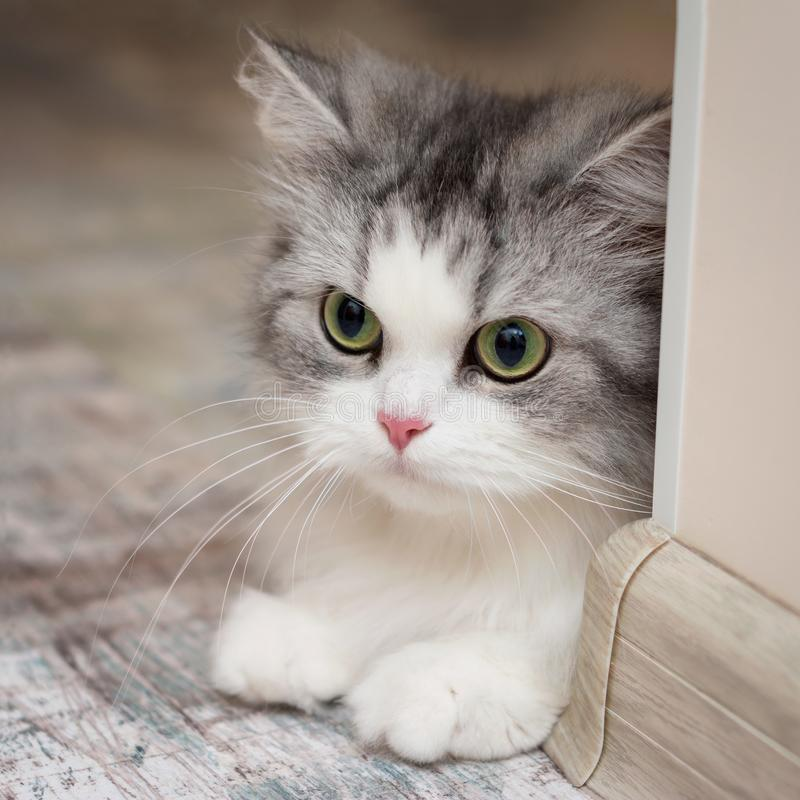
\includegraphics[width=1cm]{data/cat.png}
                };

                \cnnlayer{1.36+0.3}{0}{8}{3}{n1}
                \draw[-stealth] (cat) -- ($ (n1284.south west) - (0.1, 0) $);
                \cnnlayer{2.92+0.3}{0}{6}{3}{n2}
                \draw[-stealth] ($ (n1214.south east) + (0.1, 0) $) -- ($ (n2263.south west) - (0.1, 0) $);
                \cnnlayer{4.43+0.3}{0}{6}{5}{n3}
                \draw[-stealth] ($ (n2213.south east) + (0.1, 0) $) -- ($ (n3363.south west) - (0.2, 0) $);
                \cnnlayer{5.89+0.3}{0}{4}{5}{n4}
                \draw[-stealth] ($ (n3313.south east) + (0.2, 0) $) -- ($ (n4342.south west) - (0.2, 0) $);
                \cnnlayer{7.3+0.3}{0}{4}{7}{n5}
                \draw[-stealth] ($ (n4312.south east) + (0.2, 0) $) -- ($ (n5442.south west) - (0.3, 0) $);
                \cnnlayer{8.66}{0.15}{1}{7}{n6}
                \draw[-stealth] ($ (n5412.south east) + (0.3, 0) $) -- ($ (n6411.south west) - (0, 0) $);

                \node[circle, draw=black, fill=nodefill, text depth=0, inner sep=2pt] (y1) at (9.32, 0.275) {\tiny{$y_0$}};
                \node[circle, draw=black, fill=nodefill, text depth=0, inner sep=2pt] (y2) at (9.57, 0.025) {\tiny{$y_1$}};

                \only<1>{
                    \foreach \n in {1,...,7}{
                        \draw[-stealth] (n6\n11) -- (y1);
                        \draw[-stealth] (n6\n11) -- (y2);
                    }
                }
                \only<2>{
                    \foreach \n in {1,...,7}{
                        \draw[red, -stealth] (n6\n11) -- (y1);
                        \draw[red, -stealth] (n6\n11) -- (y2);
                    }
                }

                \def\operationfont{\scriptsize}
                \node[text depth=0, font=\operationfont\selectfont, anchor=north] at ($(cat)!0.5!(n1244) + (0, -0.8) $) {Convolution};
                \node[text depth=0, font=\operationfont\selectfont, align=center, anchor=north] at ($(n1244)!0.5!(n2233) + (0, -0.8) $) {Pooling};
                \node[text depth=0, font=\operationfont\selectfont, anchor=north] at ($(n2233)!0.5!(n3333) + (0, -0.8) $) {Convolution};
                \node[text depth=0, font=\operationfont\selectfont, align=center, anchor=north] at ($(n3333)!0.5!(n4322) + (0, -0.8) $) {Pooling};
                \node[text depth=0, font=\operationfont\selectfont, anchor=north] at ($(n4322)!0.5!(n5422) + (0, -0.8) $) {Convolution};
                \node[text depth=0, font=\operationfont\selectfont, align=center, anchor=north] at ($(n5422)!0.5!(n6411) + (0, -0.8) $) {Pooling};


                \node[text depth=0] at ($(cat)!0.5!(n1244) + (0, -3) $) {
                    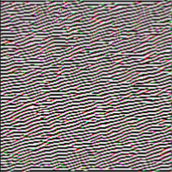
\includegraphics[height=2cm, width=2cm]{data/first.png}
                };

                \node[text depth=0] at ($(n2233)!0.5!(n3333) + (0, -3) $) {
                    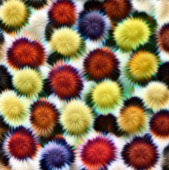
\includegraphics[height=2cm, width=2cm]{data/third.png}
                };

                \node[text depth=0] at ($(n4322)!0.5!(n5422) + (0, -3) $) {
                    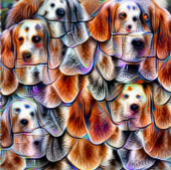
\includegraphics[height=2cm, width=2cm]{data/fifth.png}
                };
            }
            \visible<3>{
                \node[inner sep=0pt, draw=black] at (4.6, -1) {
                    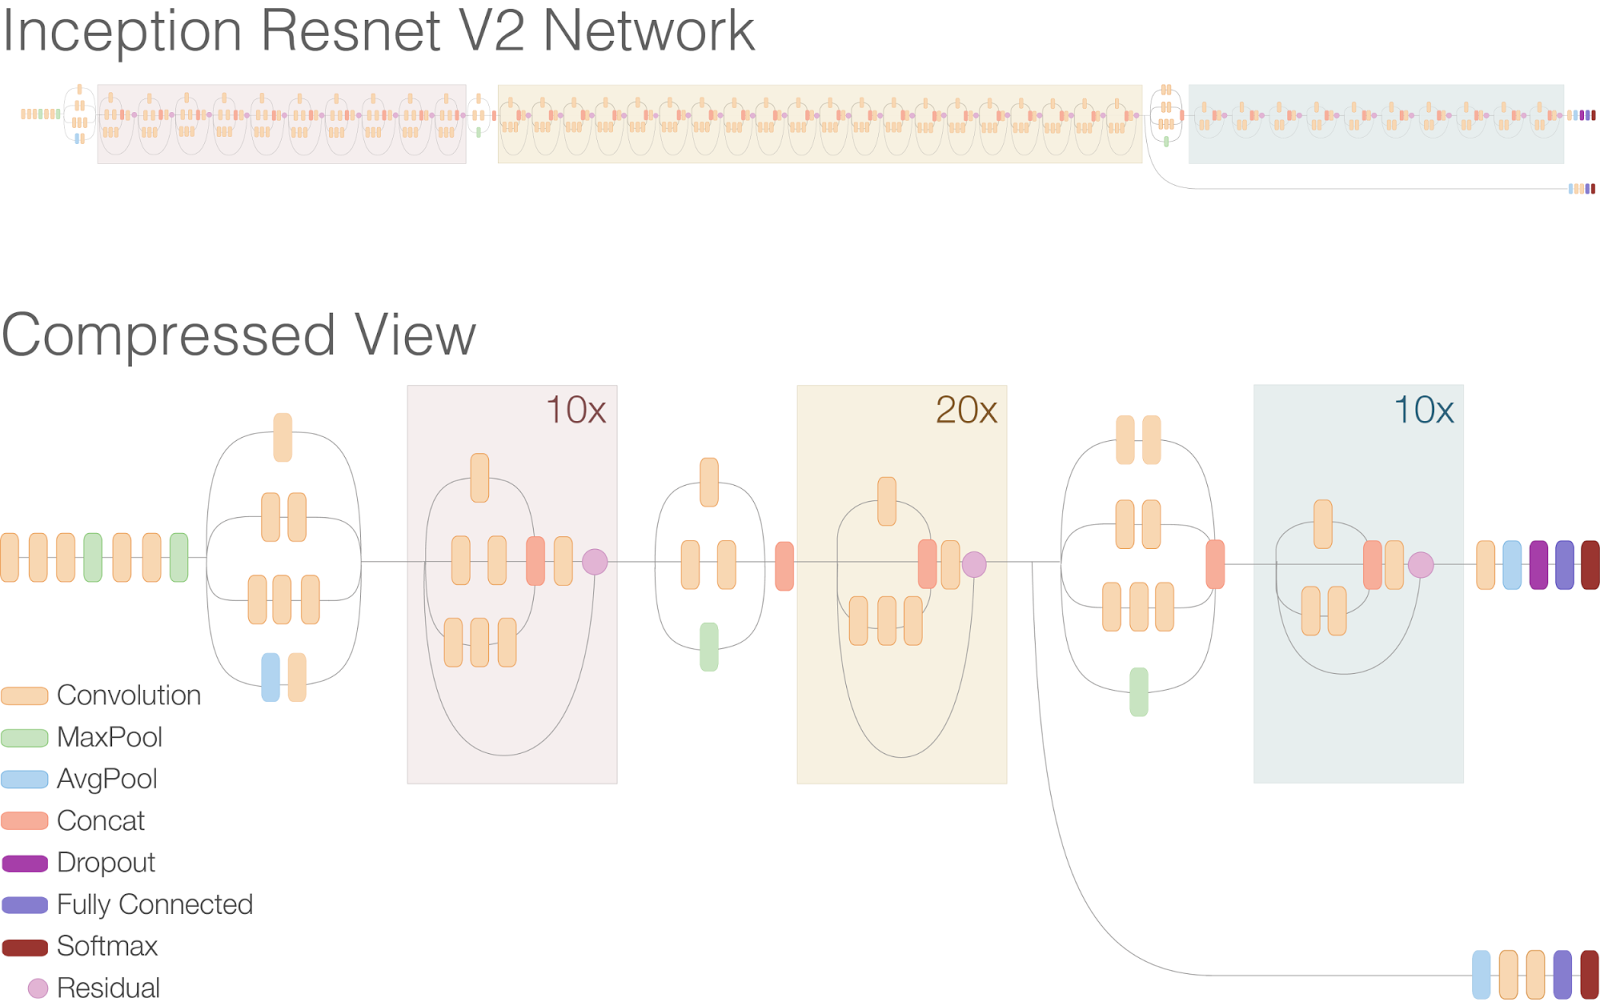
\includegraphics[width=8cm]{data/inception.png}
                };
            }
            \only<4>{
                \node[text width=10cm, align=left, font=\footnotesize\selectfont] at (4.6, -1) {
                    \underline{Convolutional neural networks (CNNs)}: Artificial neural networks tailored specifically for image data.
                    \begin{itemize}
                        \item Takes raw pixel data as input, e.g. arrays of size HxWxC
                        \item Mainly consists of convolutions and pooling operations, which lets us recognize larger and more abstract patterns the deeper we get in the model
                        \item The trainable parameters are the weights of the convolutional kernels, e.g. the patterns the model is looking for
                        \item \textbf{New architectures extend beyond this basic formula, by employing residual connections, attention mechanisms etc.}
                    \end{itemize}
                };
            }
        \end{tikzpicture}
    }
\end{frame}

\begin{frame}{Image processing: Transfer learning}
    \centering
    \resizebox{\textwidth}{!}{
        \begin{tikzpicture}
            \visible<1-5>{
                \node[circle, draw=black, fill=nodefill, text depth=0, inner sep=2pt] (y1) at (9.32, 0.275) {\tiny{$y_0$}};
                \node[circle, draw=black, fill=nodefill, text depth=0, inner sep=2pt] (y2) at (9.57, 0.025) {\tiny{$y_1$}};

                \visible<1>{
                    \node[inner sep=0pt, draw=black] (cat) at (0, 0) {
                        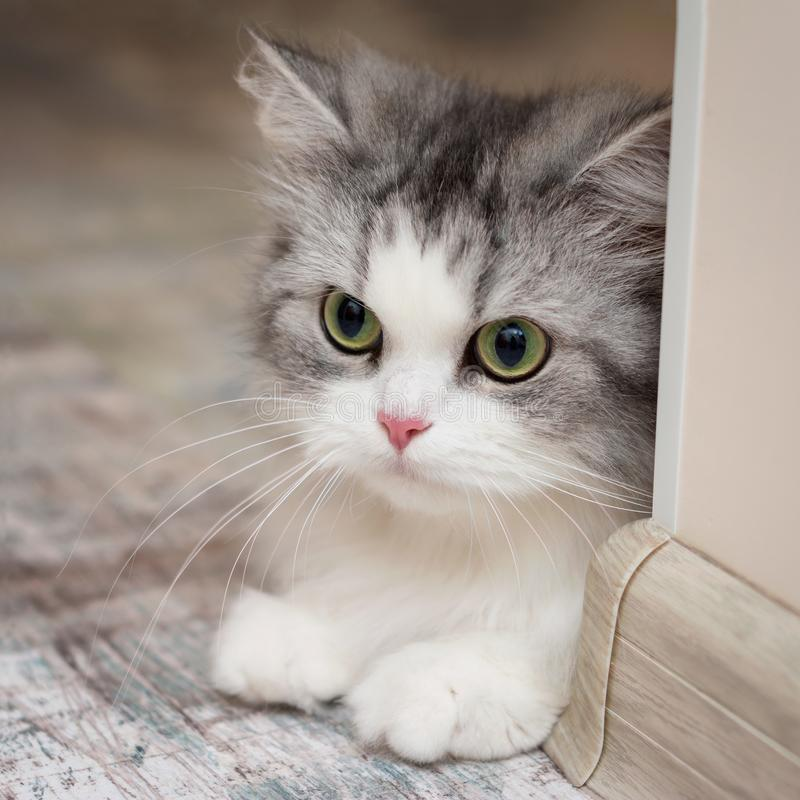
\includegraphics[width=1cm]{data/cat.png}
                    };
                    \node[anchor=west] at (y1.east) {\tiny{cat}};
                    \node[anchor=west] at (y2.east) {\tiny{dog}};
                }
                \visible<2-5>{
                    \node[inner sep=0pt, draw=black] (cat) at (0, 0) {
                        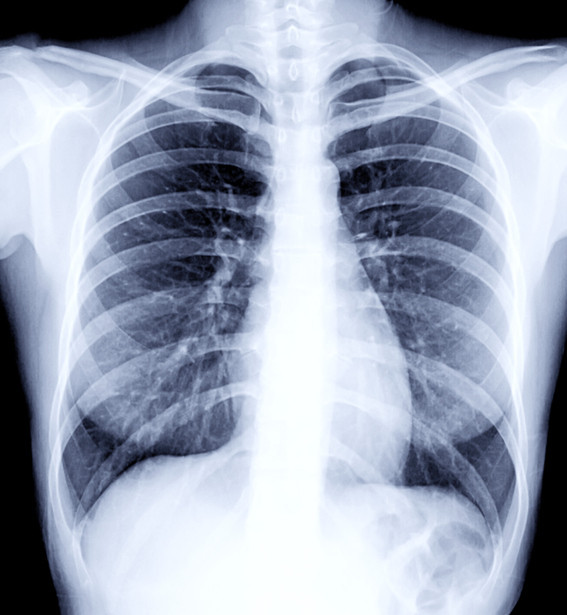
\includegraphics[width=1cm]{data/xray.jpg}
                    };
                    \node[anchor=west] at (y1.east) {\tiny{benign}};
                    \node[anchor=west] at (y2.east) {\tiny{malignant}};
                }


                \cnnlayer{1.36+0.3}{0}{8}{3}{n1}
                \visible<1-4>{\draw[-stealth] (cat) -- ($ (n1284.south west) - (0.1, 0) $);}
                \visible<5>{\draw[-stealth,red] (cat) -- ($ (n1284.south west) - (0.1, 0) $);}
                \cnnlayer{2.92+0.3}{0}{6}{3}{n2}
                \visible<1-4>{\draw[-stealth] ($ (n1214.south east) + (0.1, 0) $) -- ($ (n2263.south west) - (0.1, 0) $);}
                \visible<5>{\draw[-stealth, red] ($ (n1214.south east) + (0.1, 0) $) -- ($ (n2263.south west) - (0.1, 0) $);}
                \cnnlayer{4.43+0.3}{0}{6}{5}{n3}
                \visible<1-2,4>{\draw[-stealth] ($ (n2213.south east) + (0.1, 0) $) -- ($ (n3363.south west) - (0.2, 0) $);}
                \visible<3,5>{\draw[-stealth,red] ($ (n2213.south east) + (0.1, 0) $) -- ($ (n3363.south west) - (0.2, 0) $);}
                \cnnlayer{5.89+0.3}{0}{4}{5}{n4}
                \visible<1-2,4>{\draw[-stealth] ($ (n3313.south east) + (0.2, 0) $) -- ($ (n4342.south west) - (0.2, 0) $);}
                \visible<3,5>{\draw[-stealth, red] ($ (n3313.south east) + (0.2, 0) $) -- ($ (n4342.south west) - (0.2, 0) $);}
                \cnnlayer{7.3+0.3}{0}{4}{7}{n5}
                \visible<1-2,4>{\draw[-stealth] ($ (n4312.south east) + (0.2, 0) $) -- ($ (n5442.south west) - (0.3, 0) $);}
                \visible<3,5>{\draw[-stealth, red] ($ (n4312.south east) + (0.2, 0) $) -- ($ (n5442.south west) - (0.3, 0) $);}
                \cnnlayer{8.66}{0.15}{1}{7}{n6}
                \visible<1-2,4>{\draw[-stealth] ($ (n5412.south east) + (0.3, 0) $) -- ($ (n6411.south west) - (0, 0) $);}
                \visible<3,5>{\draw[-stealth, red] ($ (n5412.south east) + (0.3, 0) $) -- ($ (n6411.south west) - (0, 0) $);}

                \visible<1-2,4-5>{
                    \foreach \n in {1,...,7}{
                        \draw[-stealth] (n6\n11) -- (y1);
                        \draw[-stealth] (n6\n11) -- (y2);
                    }
                }

                \node[text depth=0] at ($(cat)!0.5!(n1244) + (0, -3) $) {
                    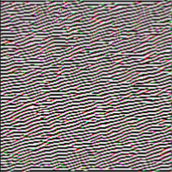
\includegraphics[height=2cm, width=2cm]{data/first.png}
                };

                \visible<1-2,4-5>{
                    \node[text depth=0] at ($(n2233)!0.5!(n3333) + (0, -3) $) {
                        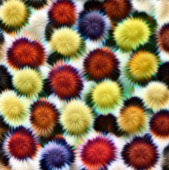
\includegraphics[height=2cm, width=2cm]{data/third.png}
                    };

                    \node[text depth=0] at ($(n4322)!0.5!(n5422) + (0, -3) $) {
                        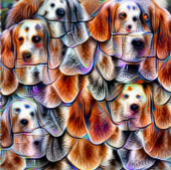
\includegraphics[height=2cm, width=2cm]{data/fifth.png}
                    };
                }

                \visible<3>{
                    \foreach \n in {1,...,7}{
                        \draw[-stealth, red] (n6\n11) -- (y1);
                        \draw[-stealth, red] (n6\n11) -- (y2);
                    }
                }
            }
            \visible<6>{
                \node[text width=10.5cm] at (4.7, -1) {
                    \underline{Transfer learning}: Utilizing pretrained models to solve new tasks.
                    \begin{itemize}
                        \item Allows us to solve tasks where we don't have enough data to train a model from scratch
                        \item Common to either freeze the weights of the convolutional part of the pre-trained model and train a new classifier on top of them, or to finetune the entire model
                    \end{itemize}
                };
            }
            \visible<7>{
                \node[] at (4.7, -1) {
                    \url{https://keras.io/api/applications/}
                };
            }
        \end{tikzpicture}
    }
\end{frame}

\begin{frame}{Image processing: Data augmentation}
    \centering
    \begin{tikzpicture}
    \visible<1-3>{
        \node[inner sep=0pt, draw=black] (orig) at (-3, 0) {
            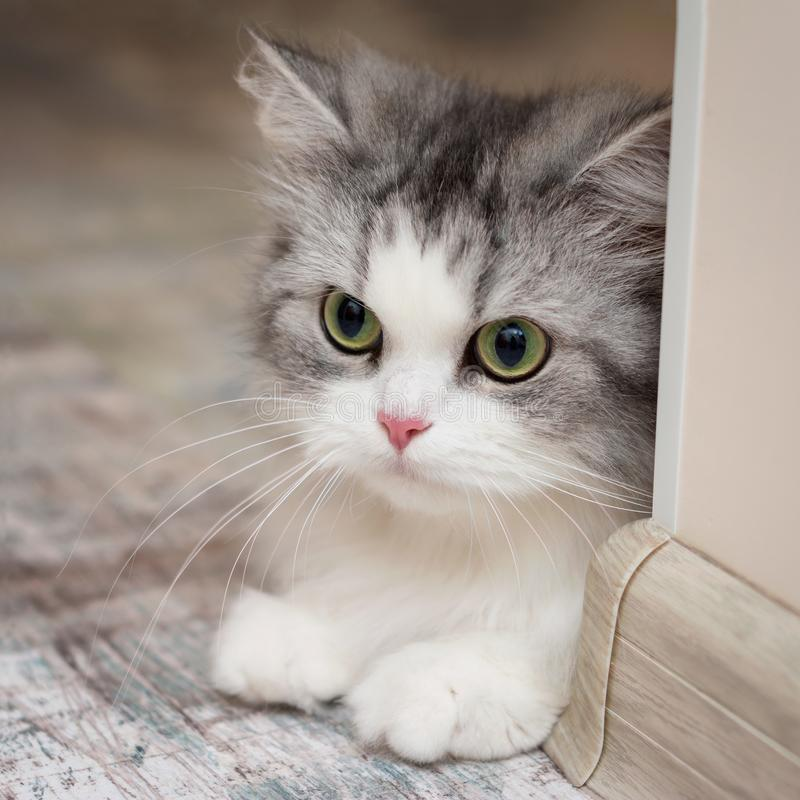
\includegraphics[width=3cm]{data/cat.png}
        };
    }
    \visible<2>{
        \node[inner sep=0pt, draw=black] (rotate) at (3, 2.5) {
            \rotatebox[origin=c]{90}{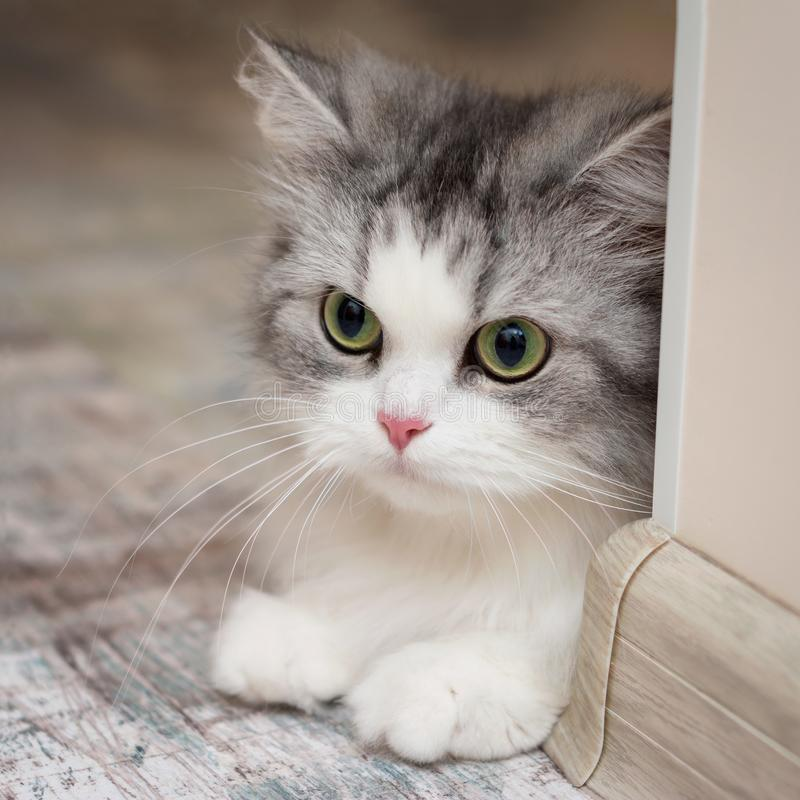
\includegraphics[width=2cm]{data/cat.png}}
        };
        \node[inner sep=0pt, draw=black] (flip) at (3, 0) {
            \scalebox{-1}[1]{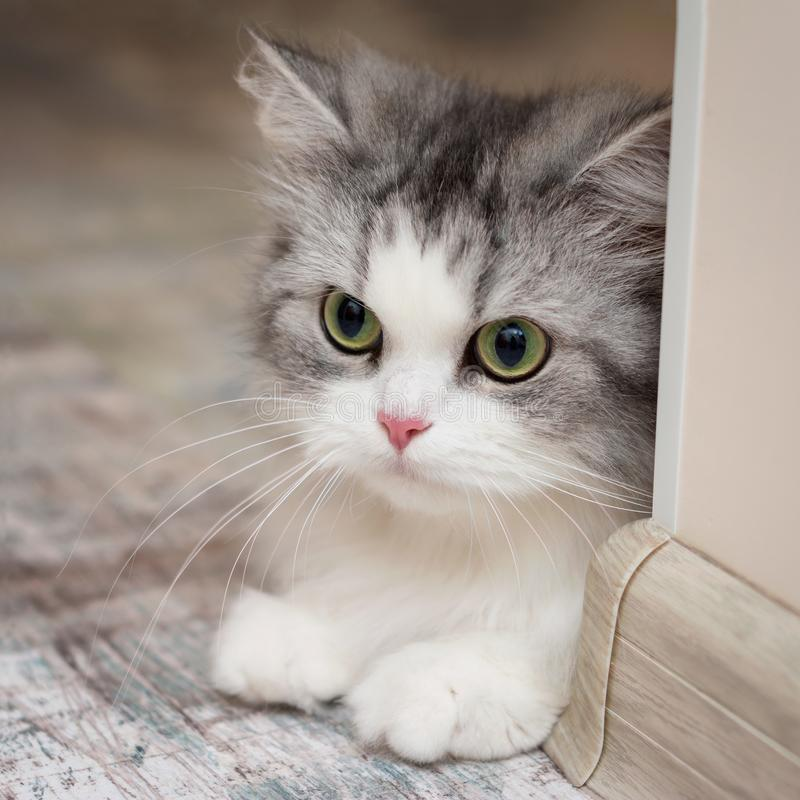
\includegraphics[width=2cm]{data/cat.png}}
        };
        \node[inner sep=0pt, draw=black] (zoom) at (3, -2.5) {
            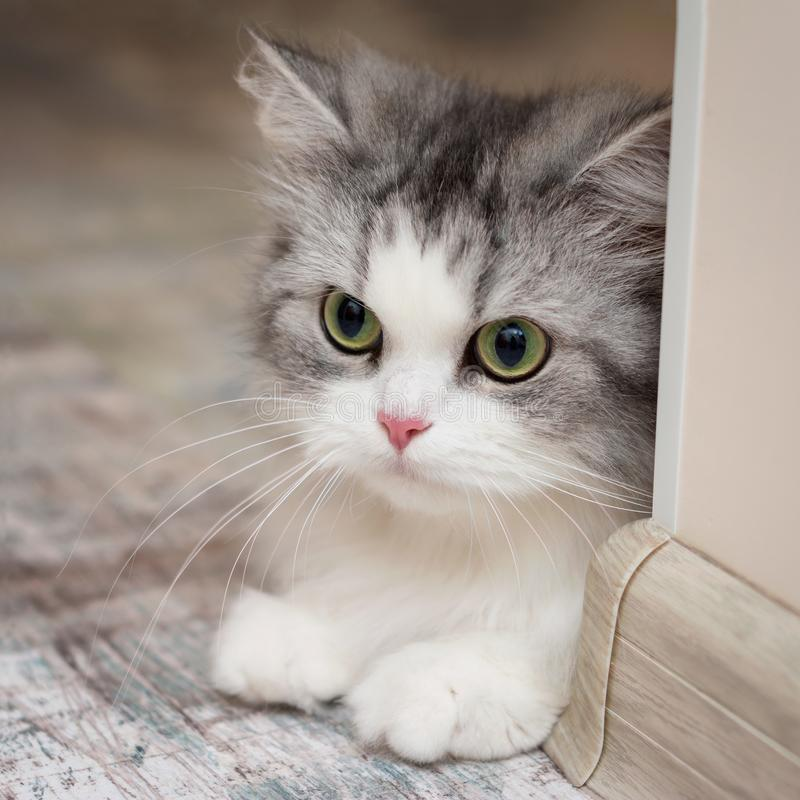
\includegraphics[
                width=2cm,
                trim={2cm 2cm 2cm 2cm},
                clip
            ]{data/cat.png}
        };

        \draw[-stealth, line width=5, blue!50] (orig) -- (rotate);
        \draw[-stealth, line width=5, blue!50] (orig) -- (flip);
        \draw[-stealth, line width=5, blue!50] (orig) -- (zoom);
    }
    \visible<3>{
        \node[inner sep=0pt, draw=black] (zoom) at (3, 0) {
            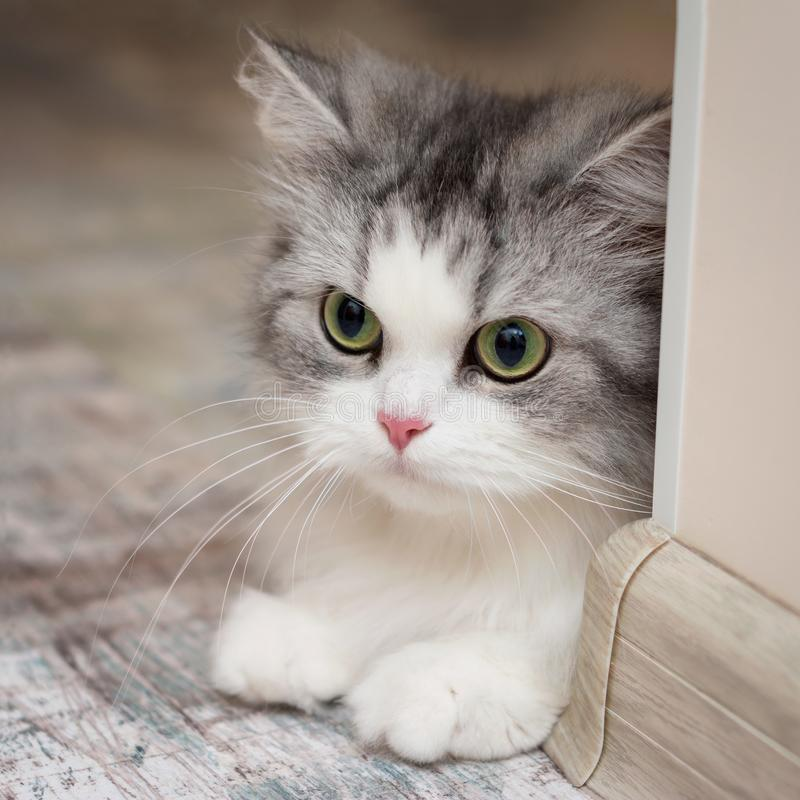
\includegraphics[
                width=3cm,
                trim={4.5cm 0.5cm 0.5cm 4.5cm},
                clip
            ]{data/cat.png}
        };

        \draw[-stealth, line width=5, red!50] (orig) -- (zoom);
    }
    \visible<4>{
        \node[] at (0, 0) {
            \url{https://albumentations.ai/}
        };
    }
    \end{tikzpicture}
\end{frame}

\begin{frame}{Image processing: Tutorial}
    \centering
    \url{https://github.com/estenhl/flowers}
\end{frame}
